\documentclass[a4paper]{article}

\usepackage[utf8]{inputenc}
\usepackage[T1]{fontenc}
\usepackage[francais]{babel}

\usepackage{graphicx}
\usepackage[lofdepth,lotdepth]{subfig}
\usepackage{algorithm}
\usepackage{algorithmic}

\title{Lecture et déchiffrement d'une photo de peinture}
\author{Théo CLAYETTE -- Thibaut ETIENNE -- Arnaud SOULIER\\Université de Montpellier}
\date{6 Mars 2018}

\begin{document}

    \maketitle

    \newpage

    \section{Introduction}

        Dans le but de déchiffrer une peinture imprimée et préalablement chiffrée par un algorithme de mélange pseudo-aléatoire, il faut avant tout faire des prétraitements sur l'image pour obtenir une image contenant uniquement la représentation de la peinture et non le fond qui l'entoure.

        Les prétraitements choisis et présentés dans ce rapport sont dans l'ordre :
        \begin{itemize}
            \item la transformation en niveaux de gris
            \item la transformation en image binaire (noir et blanc)
            \item la détection des angles de la peinture sur l'image
            \item la transformation affine de la peinture
        \end{itemize}

        Une fois toutes ces opérations effectués, on peut appliquer le déchiffrement sur la peinture uniquement et obtenir la véritable \oe{}uvre. La figure \ref{fig:original} présente la photo utilisée pour tester les algorithmes présentés dans ce rapport.

        \begin{figure}[htbp]
            \begin{center}
                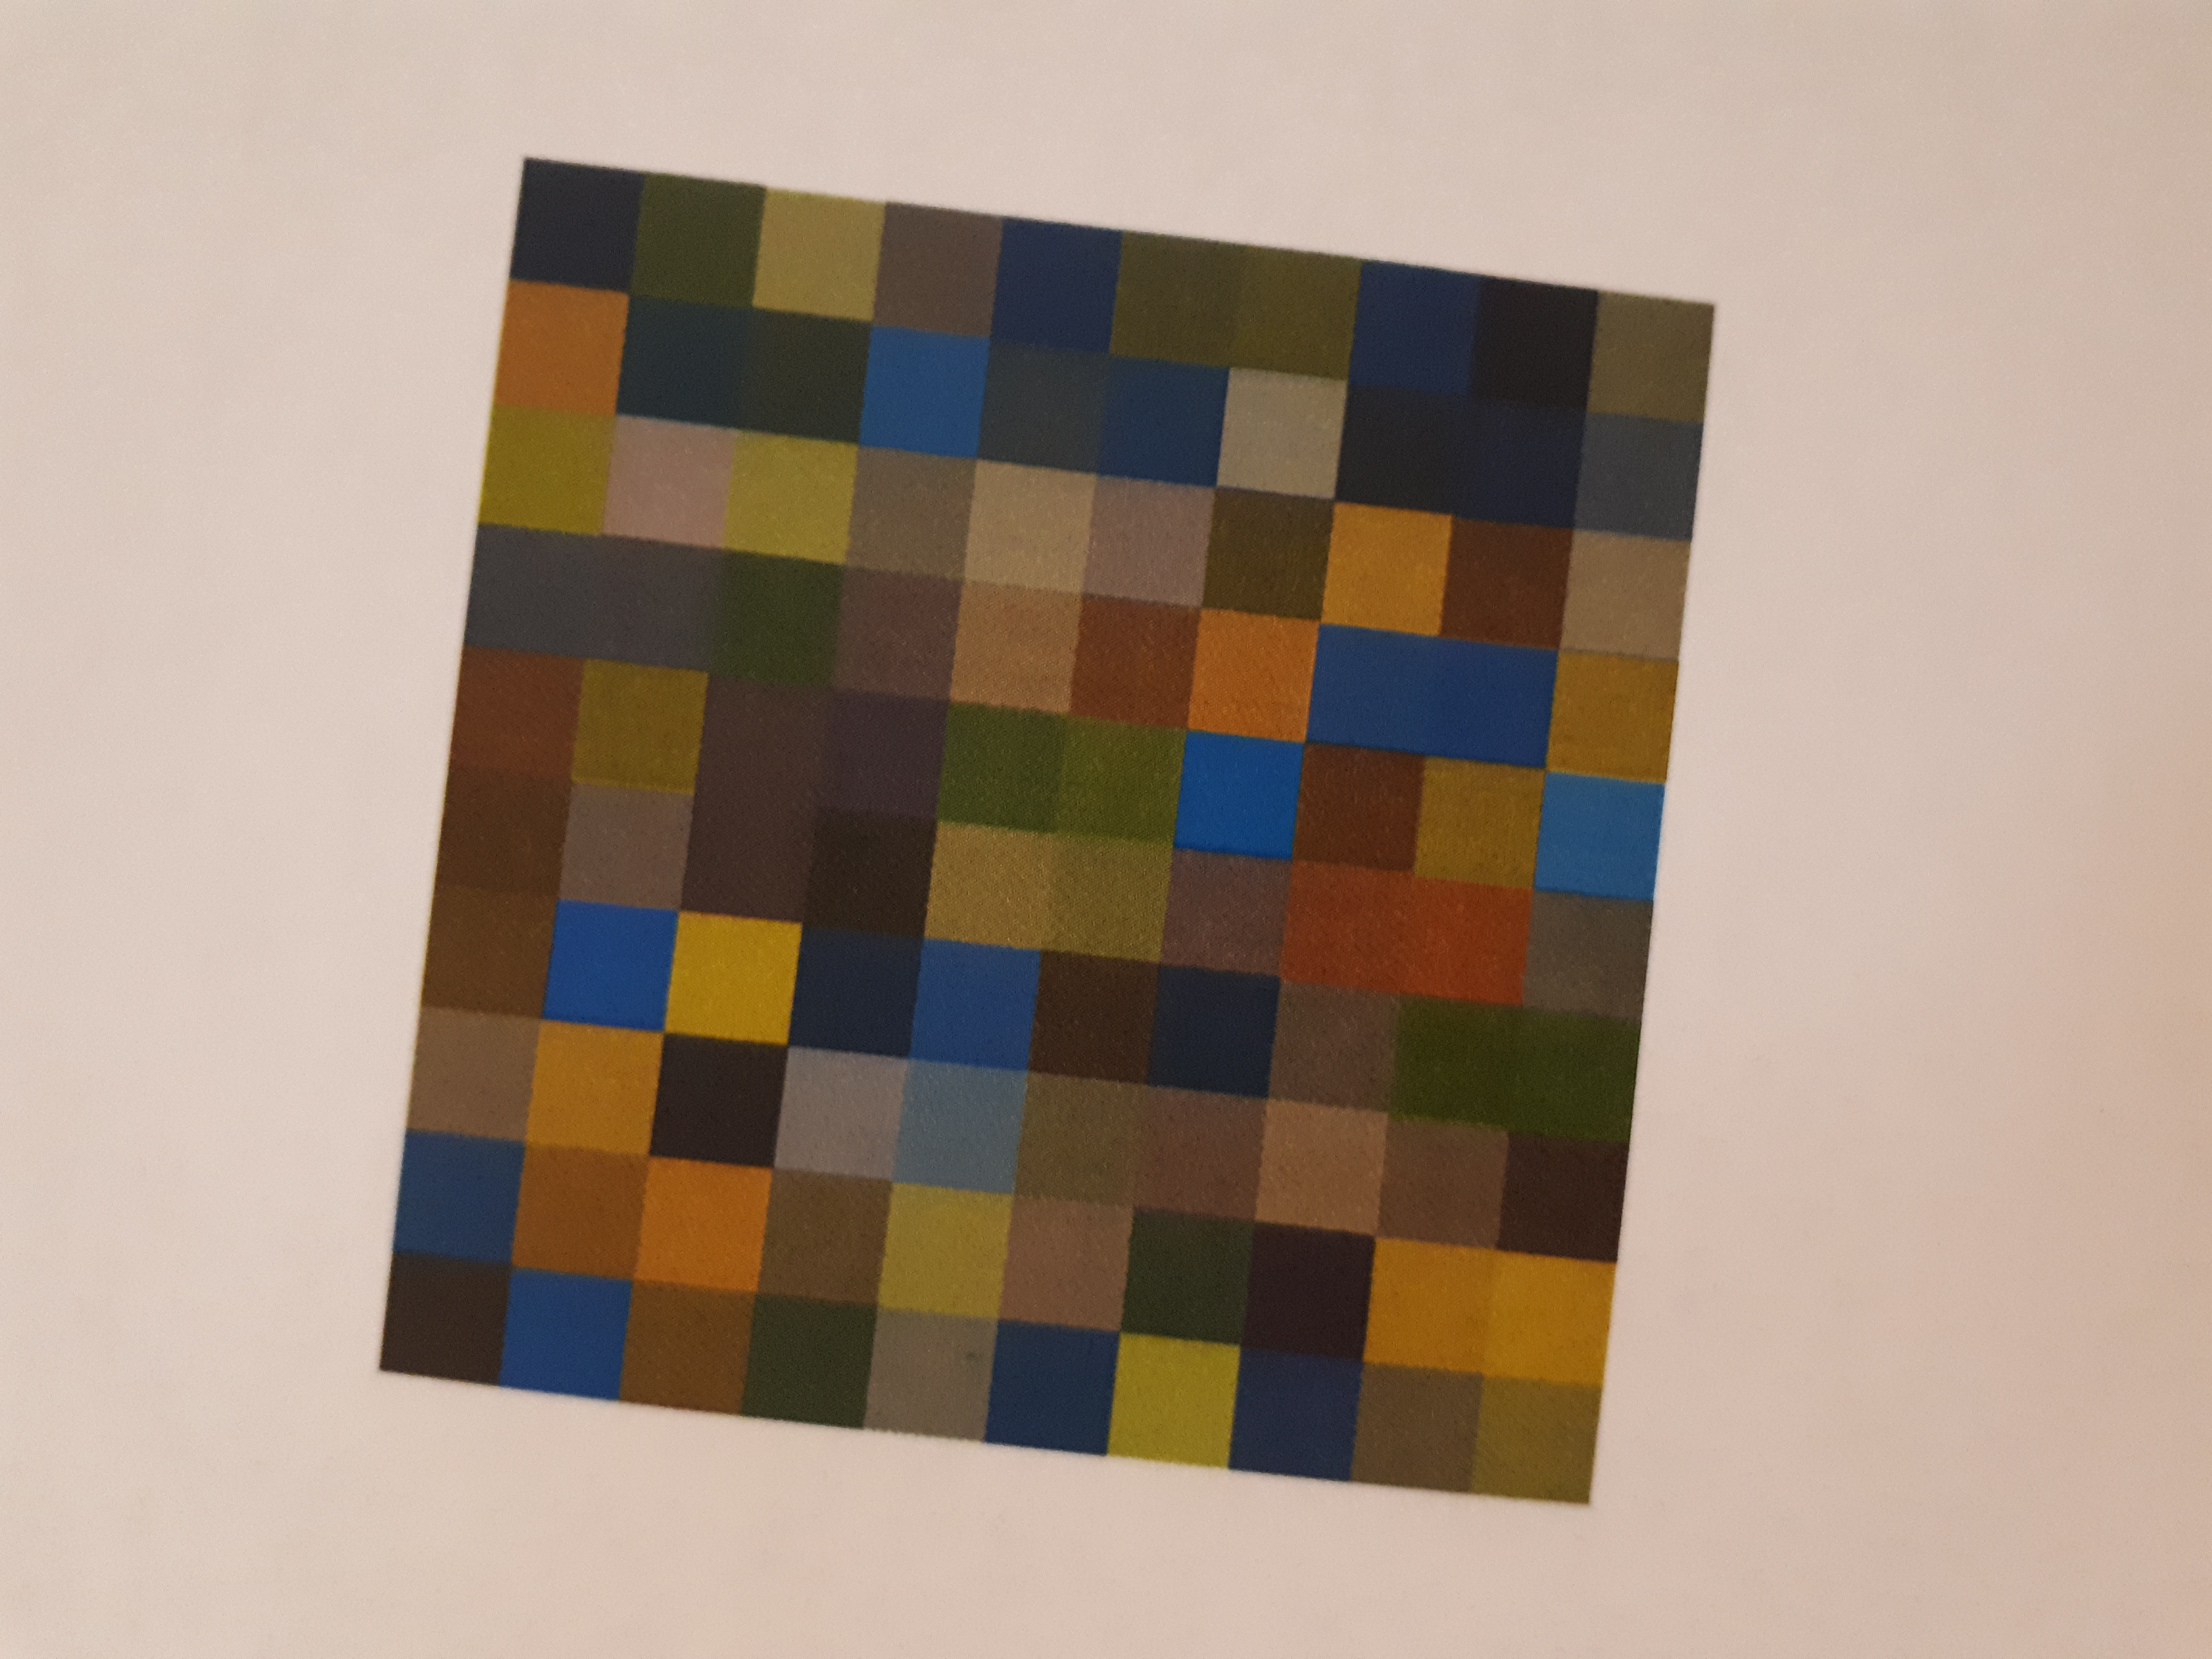
\includegraphics[width=0.3\textwidth]{rsc/vangogh.png}
                \caption{Photo utilisée pour les test de lecture et de déchiffrement d'une peinture imprimée}
                \label{fig:original}
            \end{center}
        \end{figure}

    \section{Niveaux de gris}

        La première étape de ce processus de traitement est la transformation de l'image couleur (format .ppm) en niveaux de gris (format .pgm). Pour ce faire, il suffit d'appliquer la formule suivante (cf. équation \ref{eq:gray_scale}) à tous les pixels de l'image.

        \begin{equation}
            data[i] = 0.299 \cdot R[i] + 0.587 \cdot G[i] + 0.114 \cdot B[i]
            \label{eq:gray_scale}
        \end{equation}
        avec
        \begin{itemize}
            \item $data[i]$ la valeur en niveaux de gris du pixel $i$ de l'image
            \item $R[i]$ la valeur de la composante rouge du pixel $i$ de l'image
            \item $G[i]$ la valeur de la composante verte du pixel $i$ de l'image
            \item $B[i]$ la valeur de la composante bleue du pixel $i$ de l'image
        \end{itemize}

        Il en résulte donc une image de même dimension mais composée uniquement de nuance de gris (cf. figure \ref{fig:gray}\subref{subfig:gray_res}).

        \begin{figure}[htbp]
            \begin{center}
                \subfloat[Photo originale]{
                    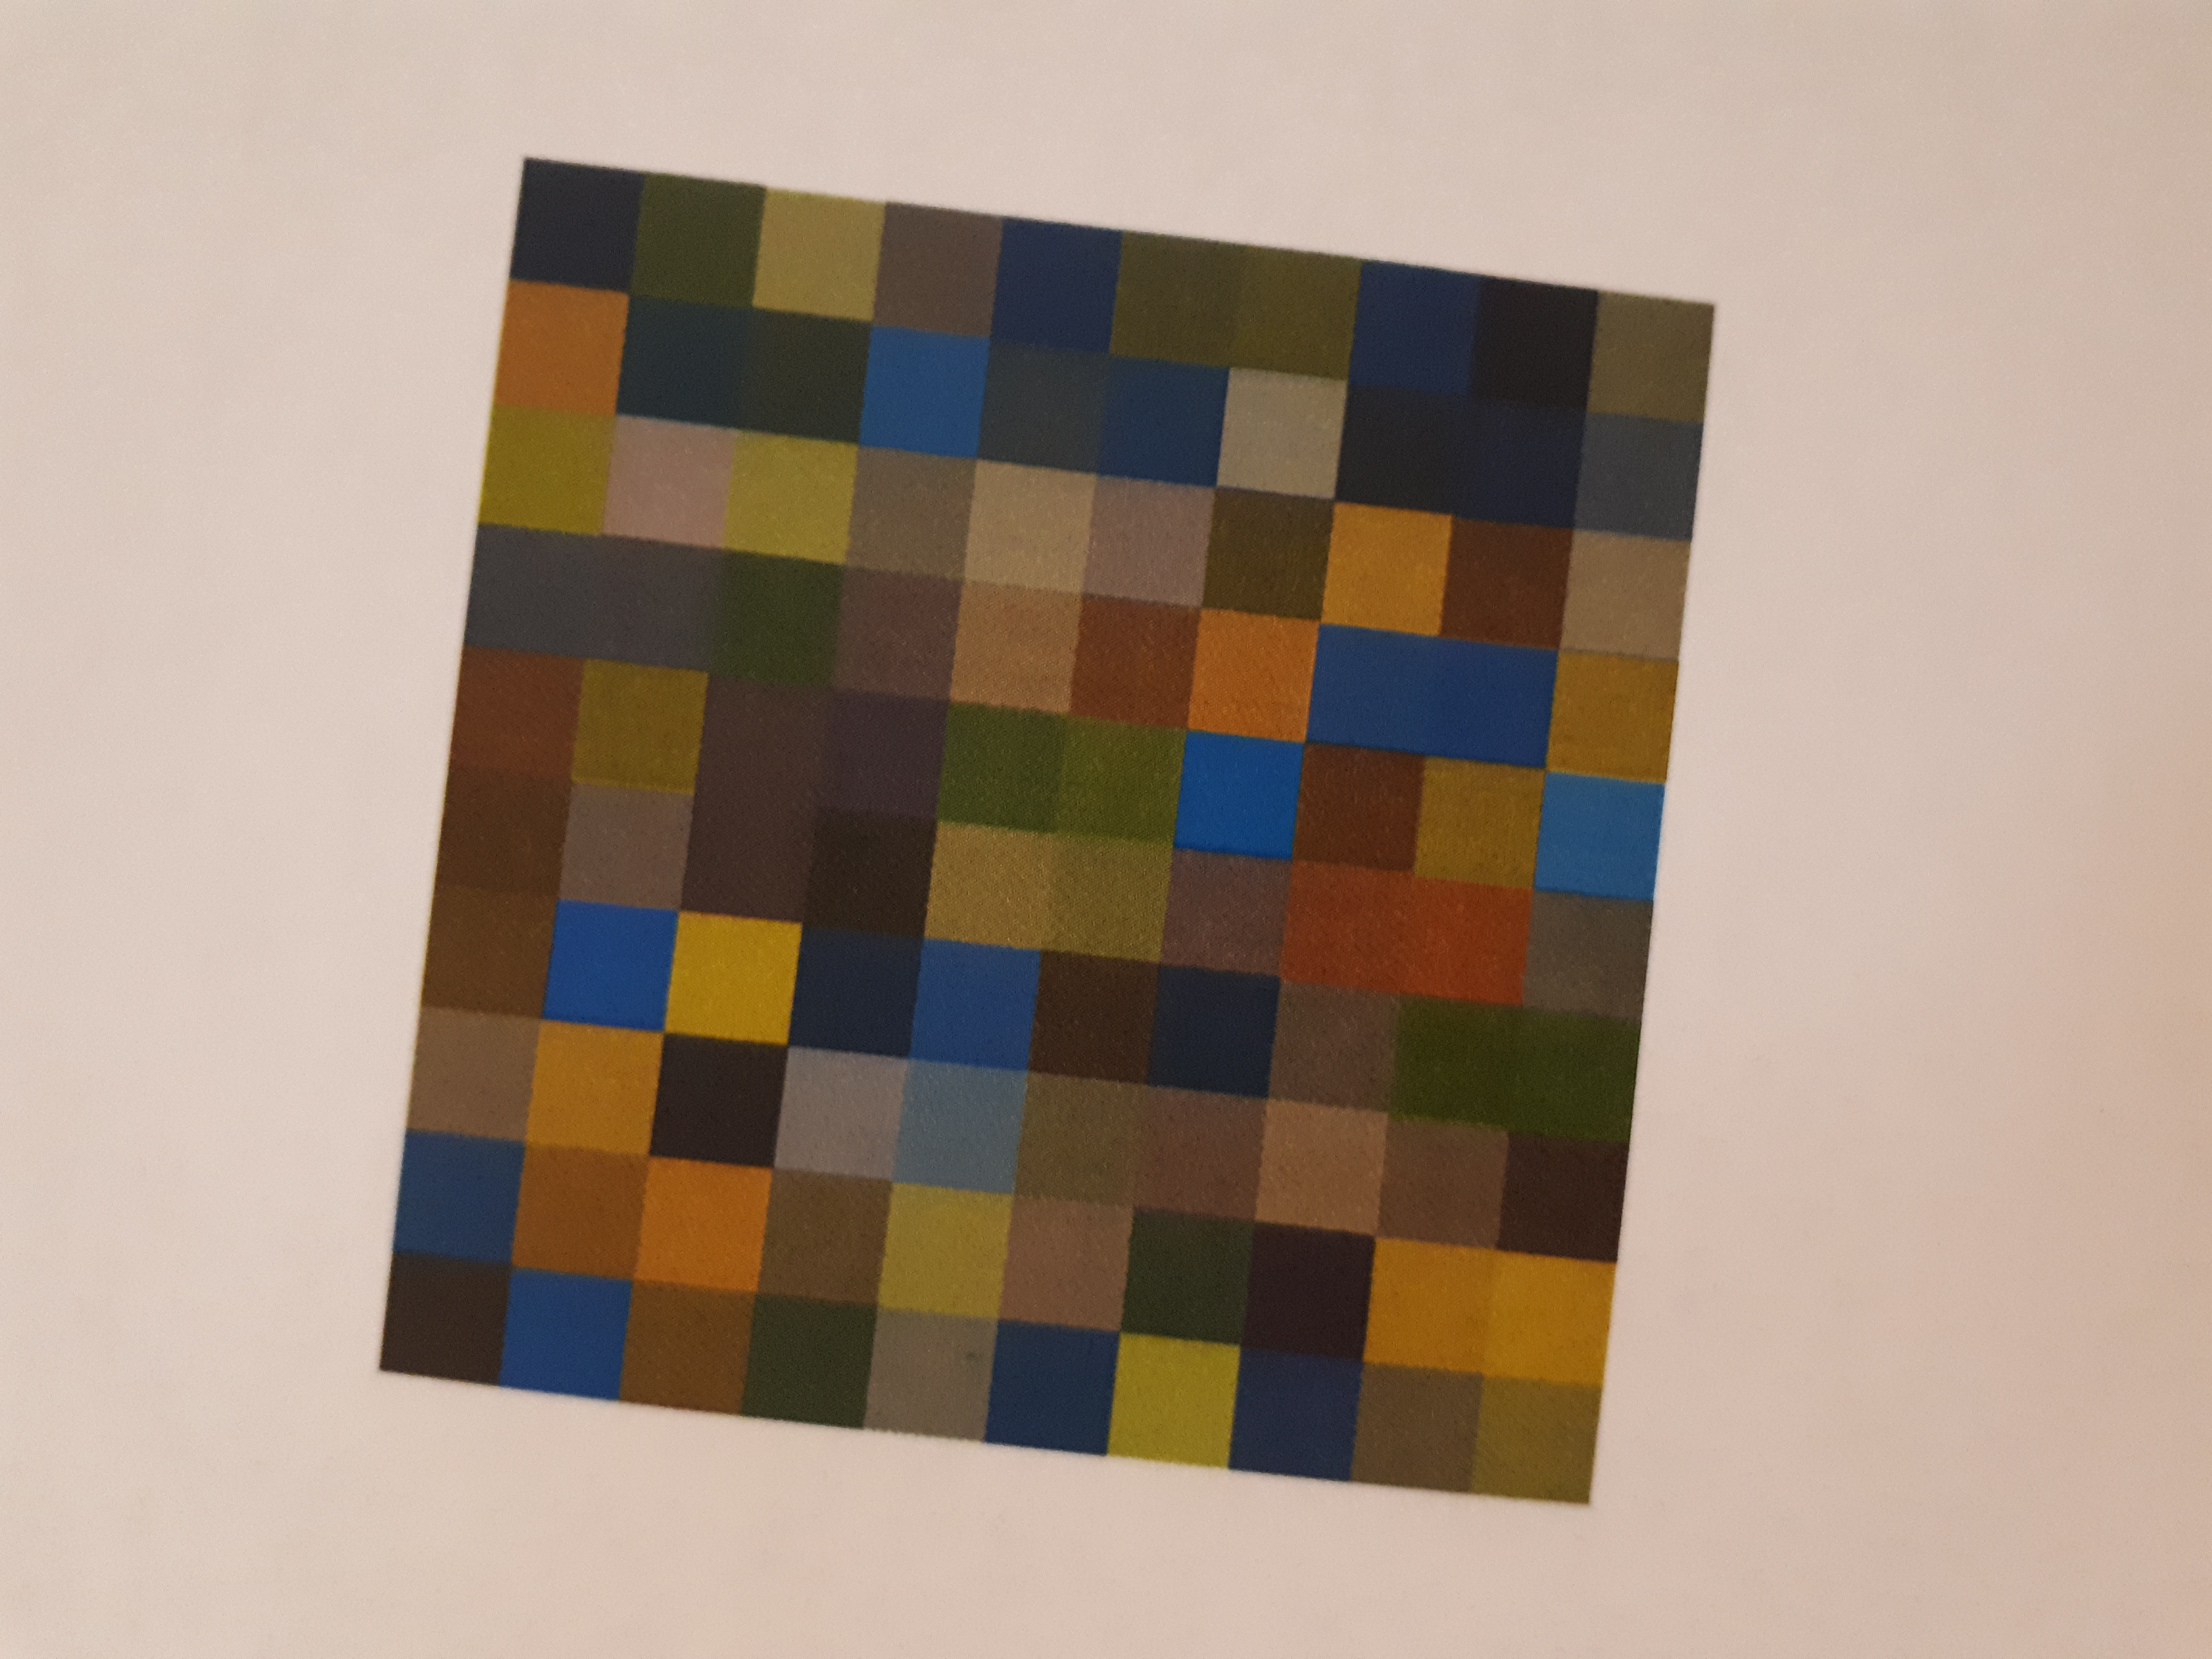
\includegraphics[width=0.3\textwidth]{rsc/vangogh.png}
                    \label{subfig:gray_original}}
                \subfloat[Photo en niveaux de gris]{
                    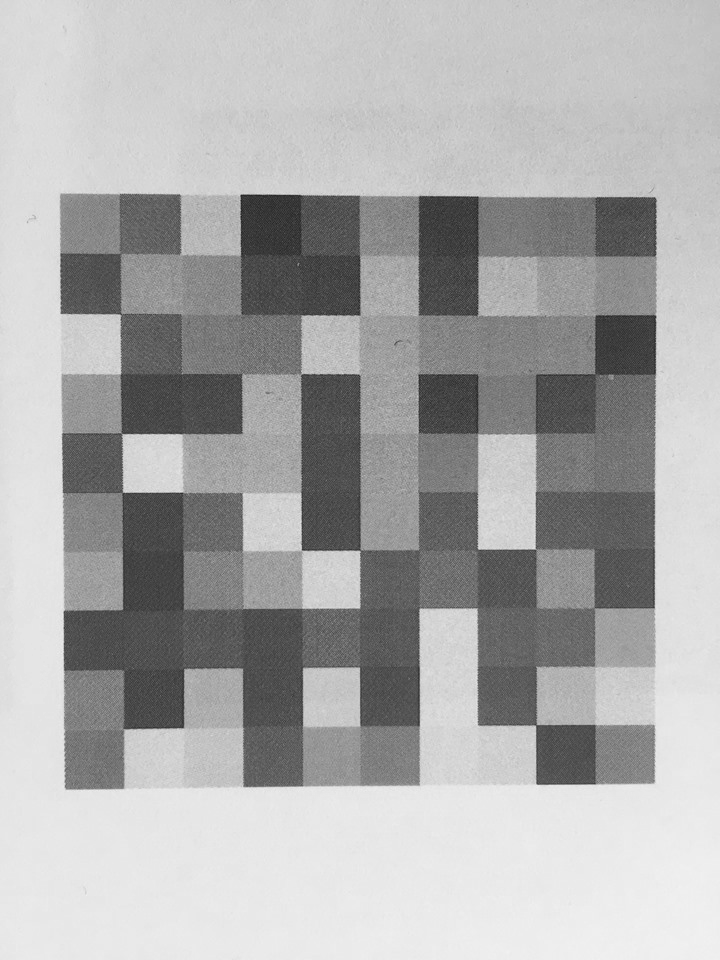
\includegraphics[width=0.3\textwidth]{rsc/grayScale.png}
                    \label{subfig:gray_res}}
                \caption{Conversion en niveaux de gris de l'image}
                \label{fig:gray}
            \end{center}
        \end{figure}

    \section{Image binaire}

        À partir de l'image en nivaux de gris, on passe à une image binaire (noir et blanc) avec un simple seuillage des valeurs. Pour chaque pixel de l'image, si sa valeur est supérieure au seuil choisi, alors cette valeur devient 255 (blanc). Si sa valeur est inférieure au seuil choisi, alors cette valeur devient 0 (noir).

        La figure \ref{fig:binary}\subref{subfig:binary_res} montre le résultat de la conversion binaire de l'image en niveaux de gris.

        \begin{figure}[htbp]
            \begin{center}
                \subfloat[Photo en niveaux de gris originale]{
                    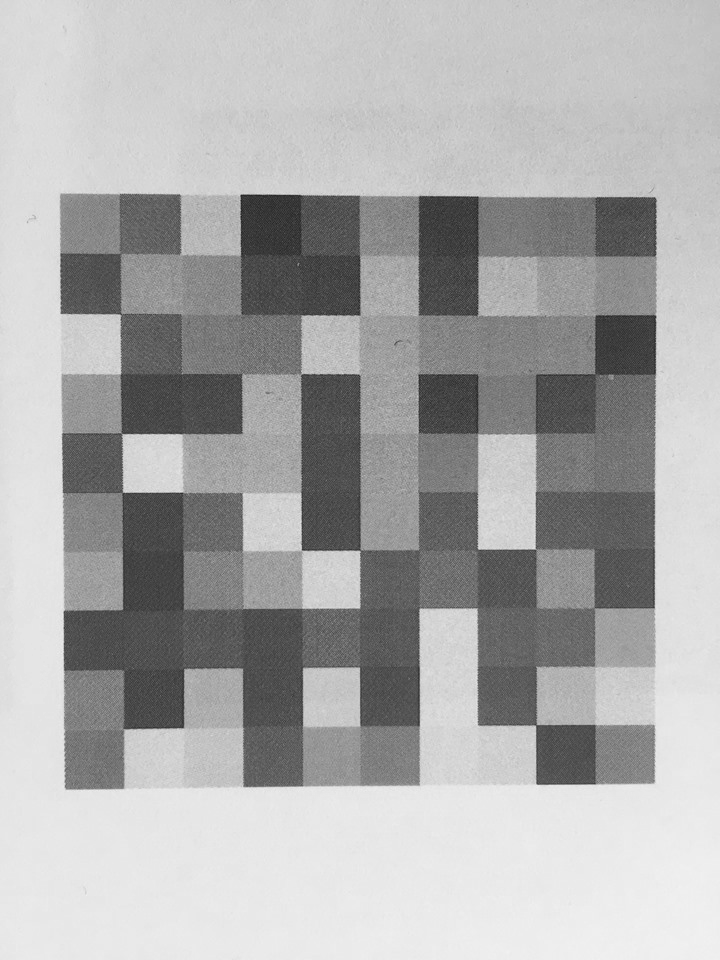
\includegraphics[width=0.3\textwidth]{rsc/grayScale.png}
                    \label{subfig:binary_gray}}
                \subfloat[Histogramme de la photo en niveaux de gris]{
                    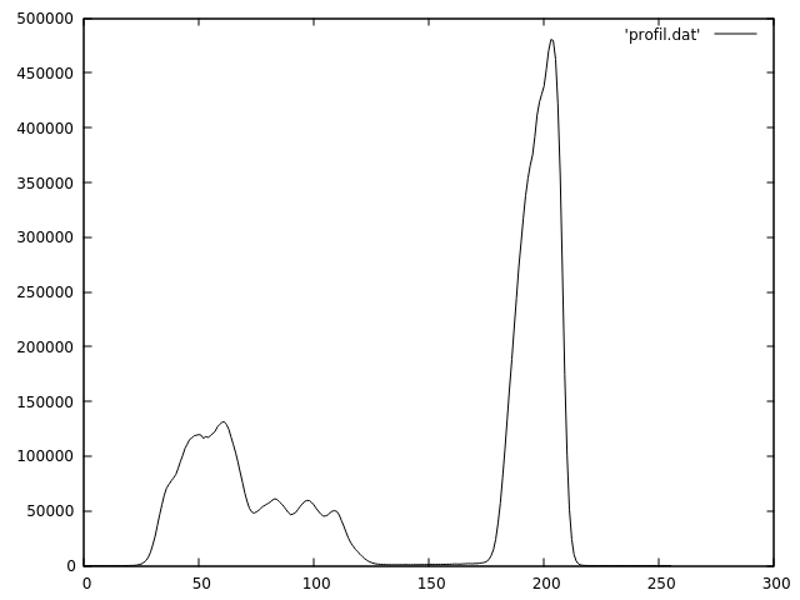
\includegraphics[width=0.3\textwidth]{rsc/histo.png}
                    \label{subfig:binary_histo}}
                \subfloat[Photo binaire (seuil 120)]{
                    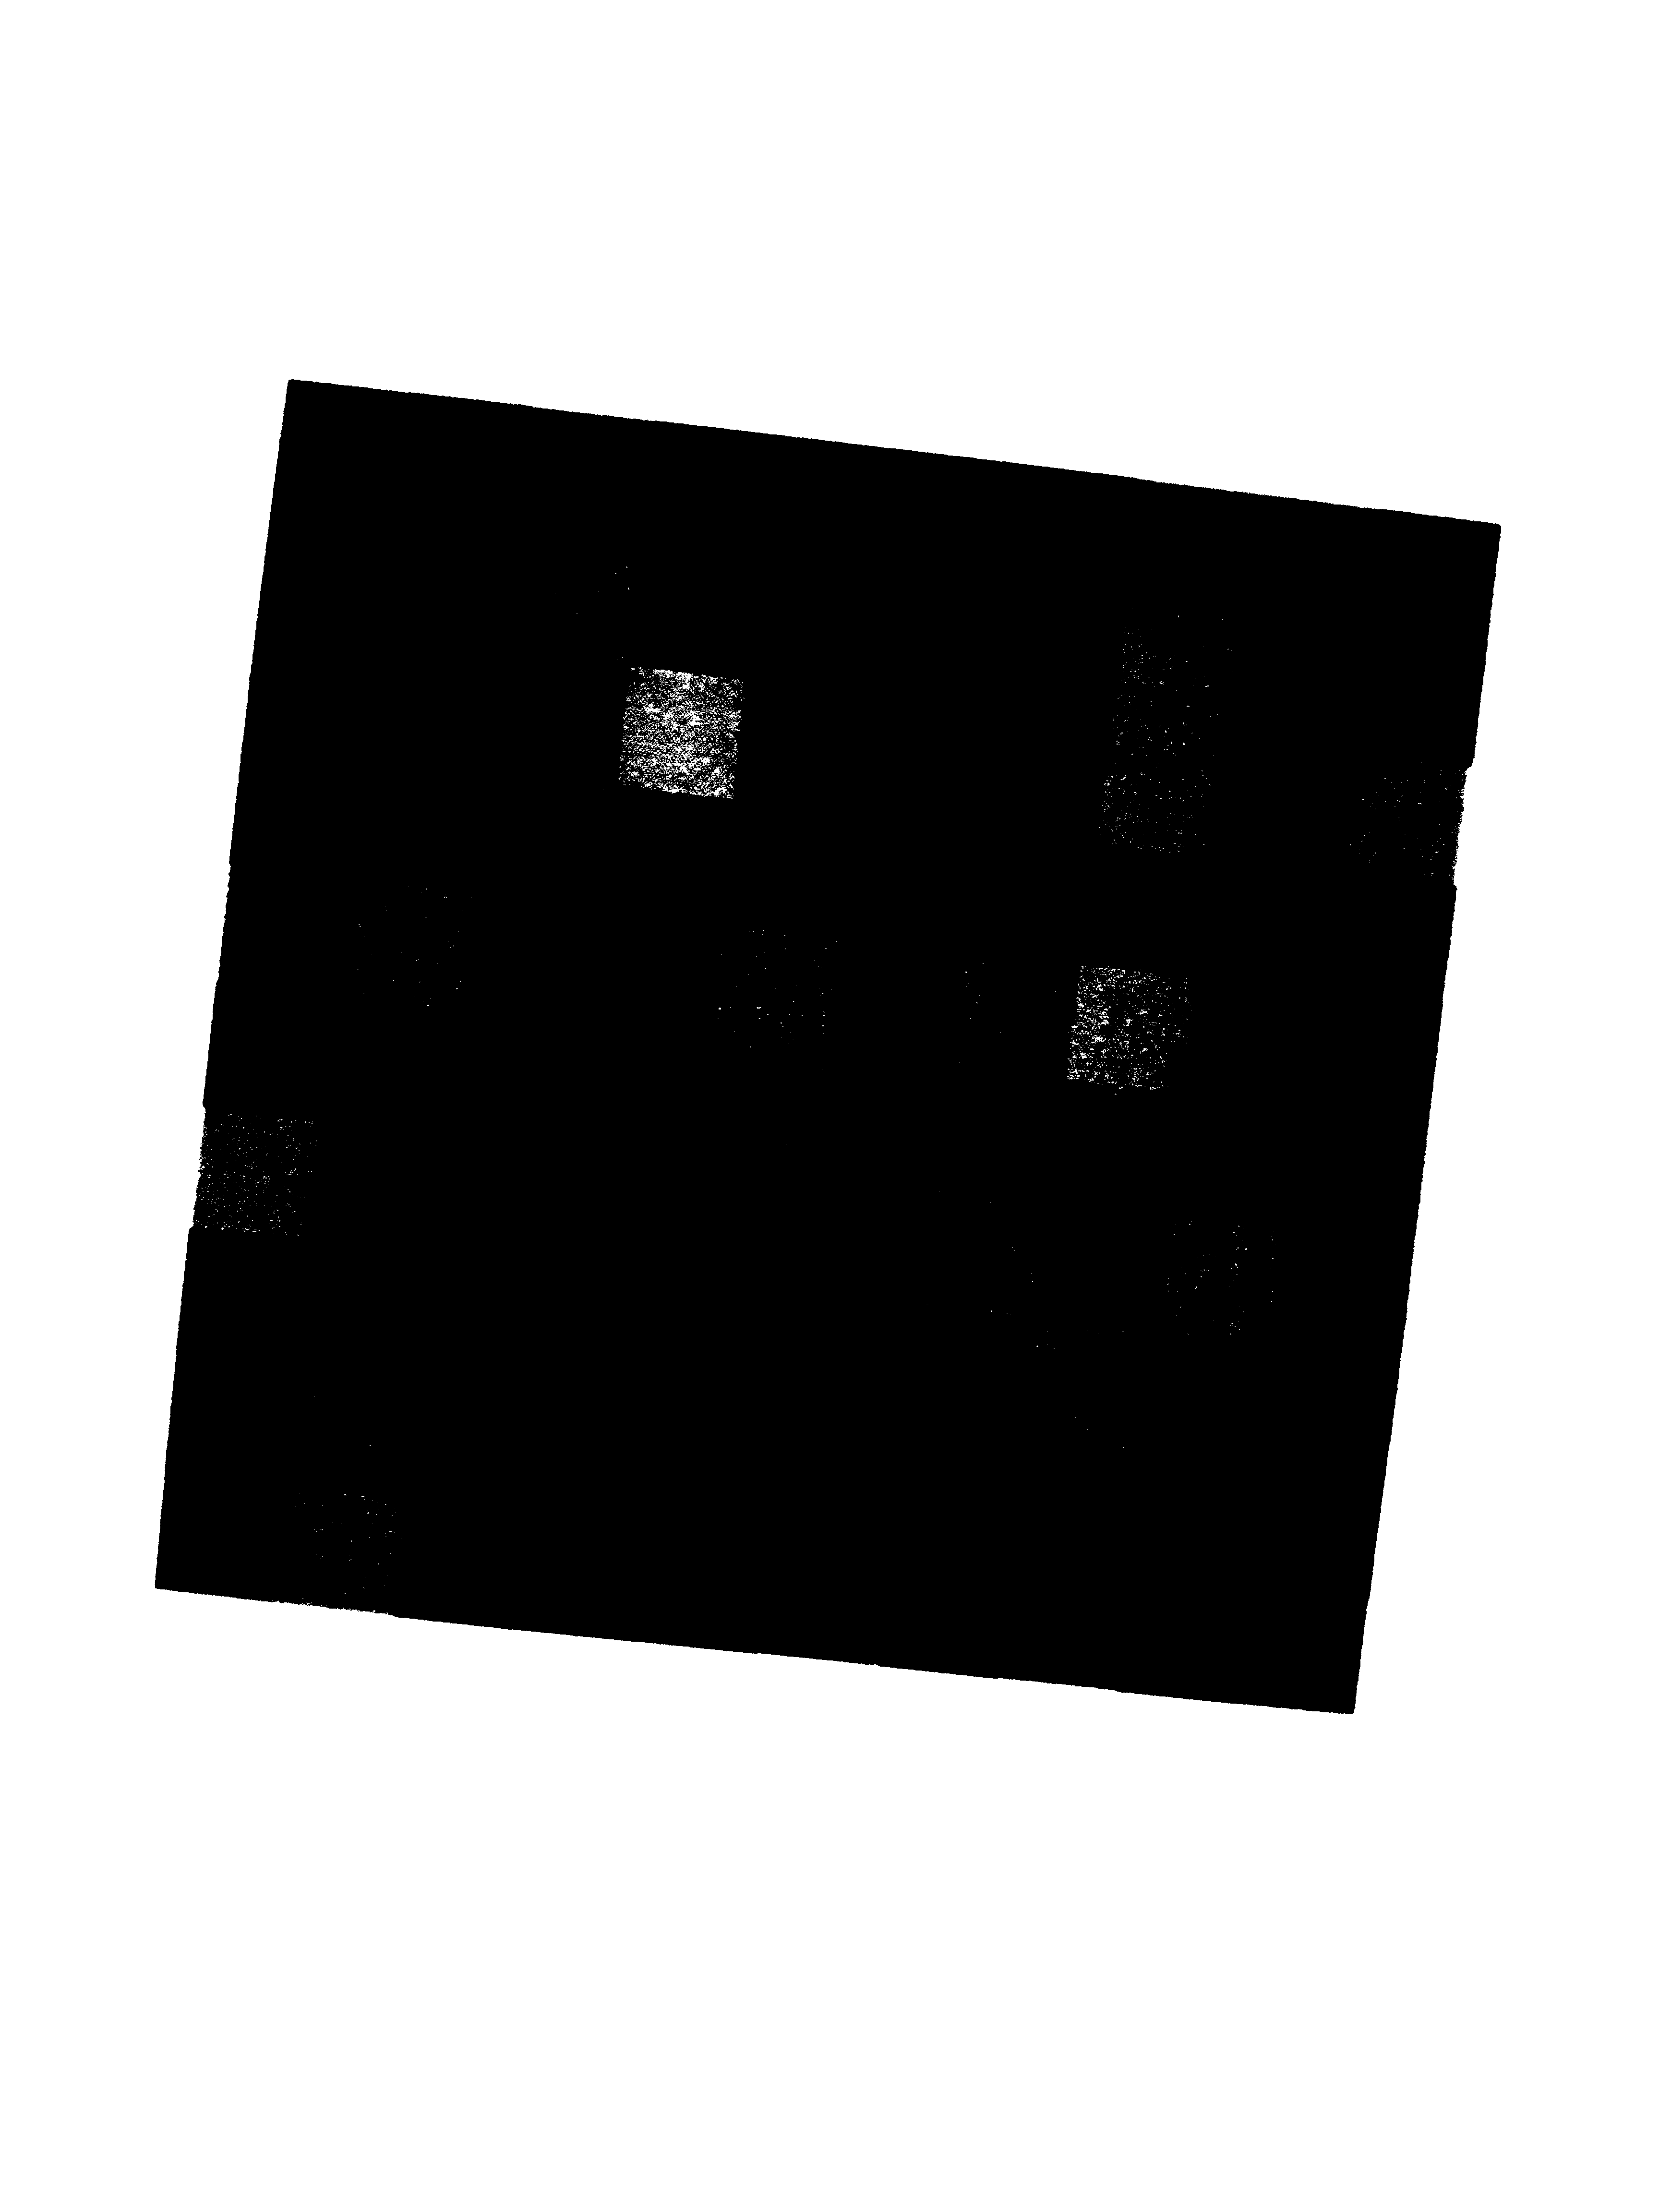
\includegraphics[width=0.3\textwidth]{rsc/binary.png}
                    \label{subfig:binary_res}}
                \caption{Conversion en binaire de l'image}
                \label{fig:binary}
            \end{center}
        \end{figure}

        Pour obtenir la valeur de seuillage à utiliser pour faire cette conversion, il faut observer l'histogramme des valeurs de l'image en niveaux de gris et choisir une valeur cohérente (séparation nette entre les pixels les plus foncés et les plus clairs). On peut également automatiser ce choix en prenant par exemple la première valeur telle que 40\% des pixels ont une valeur inférieure à ce choix.

    \section{Détection des angles}

        À partir de l'image binaire, la détection des angles est grandement facilité grace aux faibles nombres de valeur possible (noir ou blanc) et la répartition séparée dans l'image.

        L'algorithme utilisé ici part à tour de rôle des angles de l'image et parcours tous les pixels dans une zone entre cet angle et le centre de l'image à la recherche du pixel noir le plus proche de l'angle. Ce pixel sera alors l'angle de la peinture sur l'image. L'algo \ref{algo:findAngle} représente l'itération d'un des angles. Il doit donc être reproduit et adapté trois fois pour retourner les quatre angles.

        \begin{algorithm}
            \begin{algorithmic}
                \STATE $x \leftarrow height / 2$
                \STATE $y \leftarrow width / 2$
                \FOR{$i\ 0..height/2$}
                    \FOR{$j\ 0..widht/2$}
                        \IF{$data[i*width+j] = 0$}
                            \IF{$i + j < x + y$}
                                \STATE $x \leftarrow i$
                                \STATE $y \leftarrow j$
                            \ENDIF
                        \ENDIF
                    \ENDFOR
                \ENDFOR
            \end{algorithmic}
            \caption{Trouve l'angle supérieur gauche}
            \label{algo:findAngle}
        \end{algorithm}

        Les quatre formules pour calculer le point le plus proche de l'angle sont :
        \begin{itemize}
            \item $i + j < x + j$ pour l'angle supérieur gauche
            \item $j - i > y - x$ pour l'angle supérieur droit
            \item $i + j > x + y$ pour l'angle inférieur droit
            \item $i - j > x - y$ pour l'angle inférieur gauche
        \end{itemize}

        \begin{figure}[htbp]
            \begin{center}
                \subfloat[Photo binaire (seuil 120)]{
                    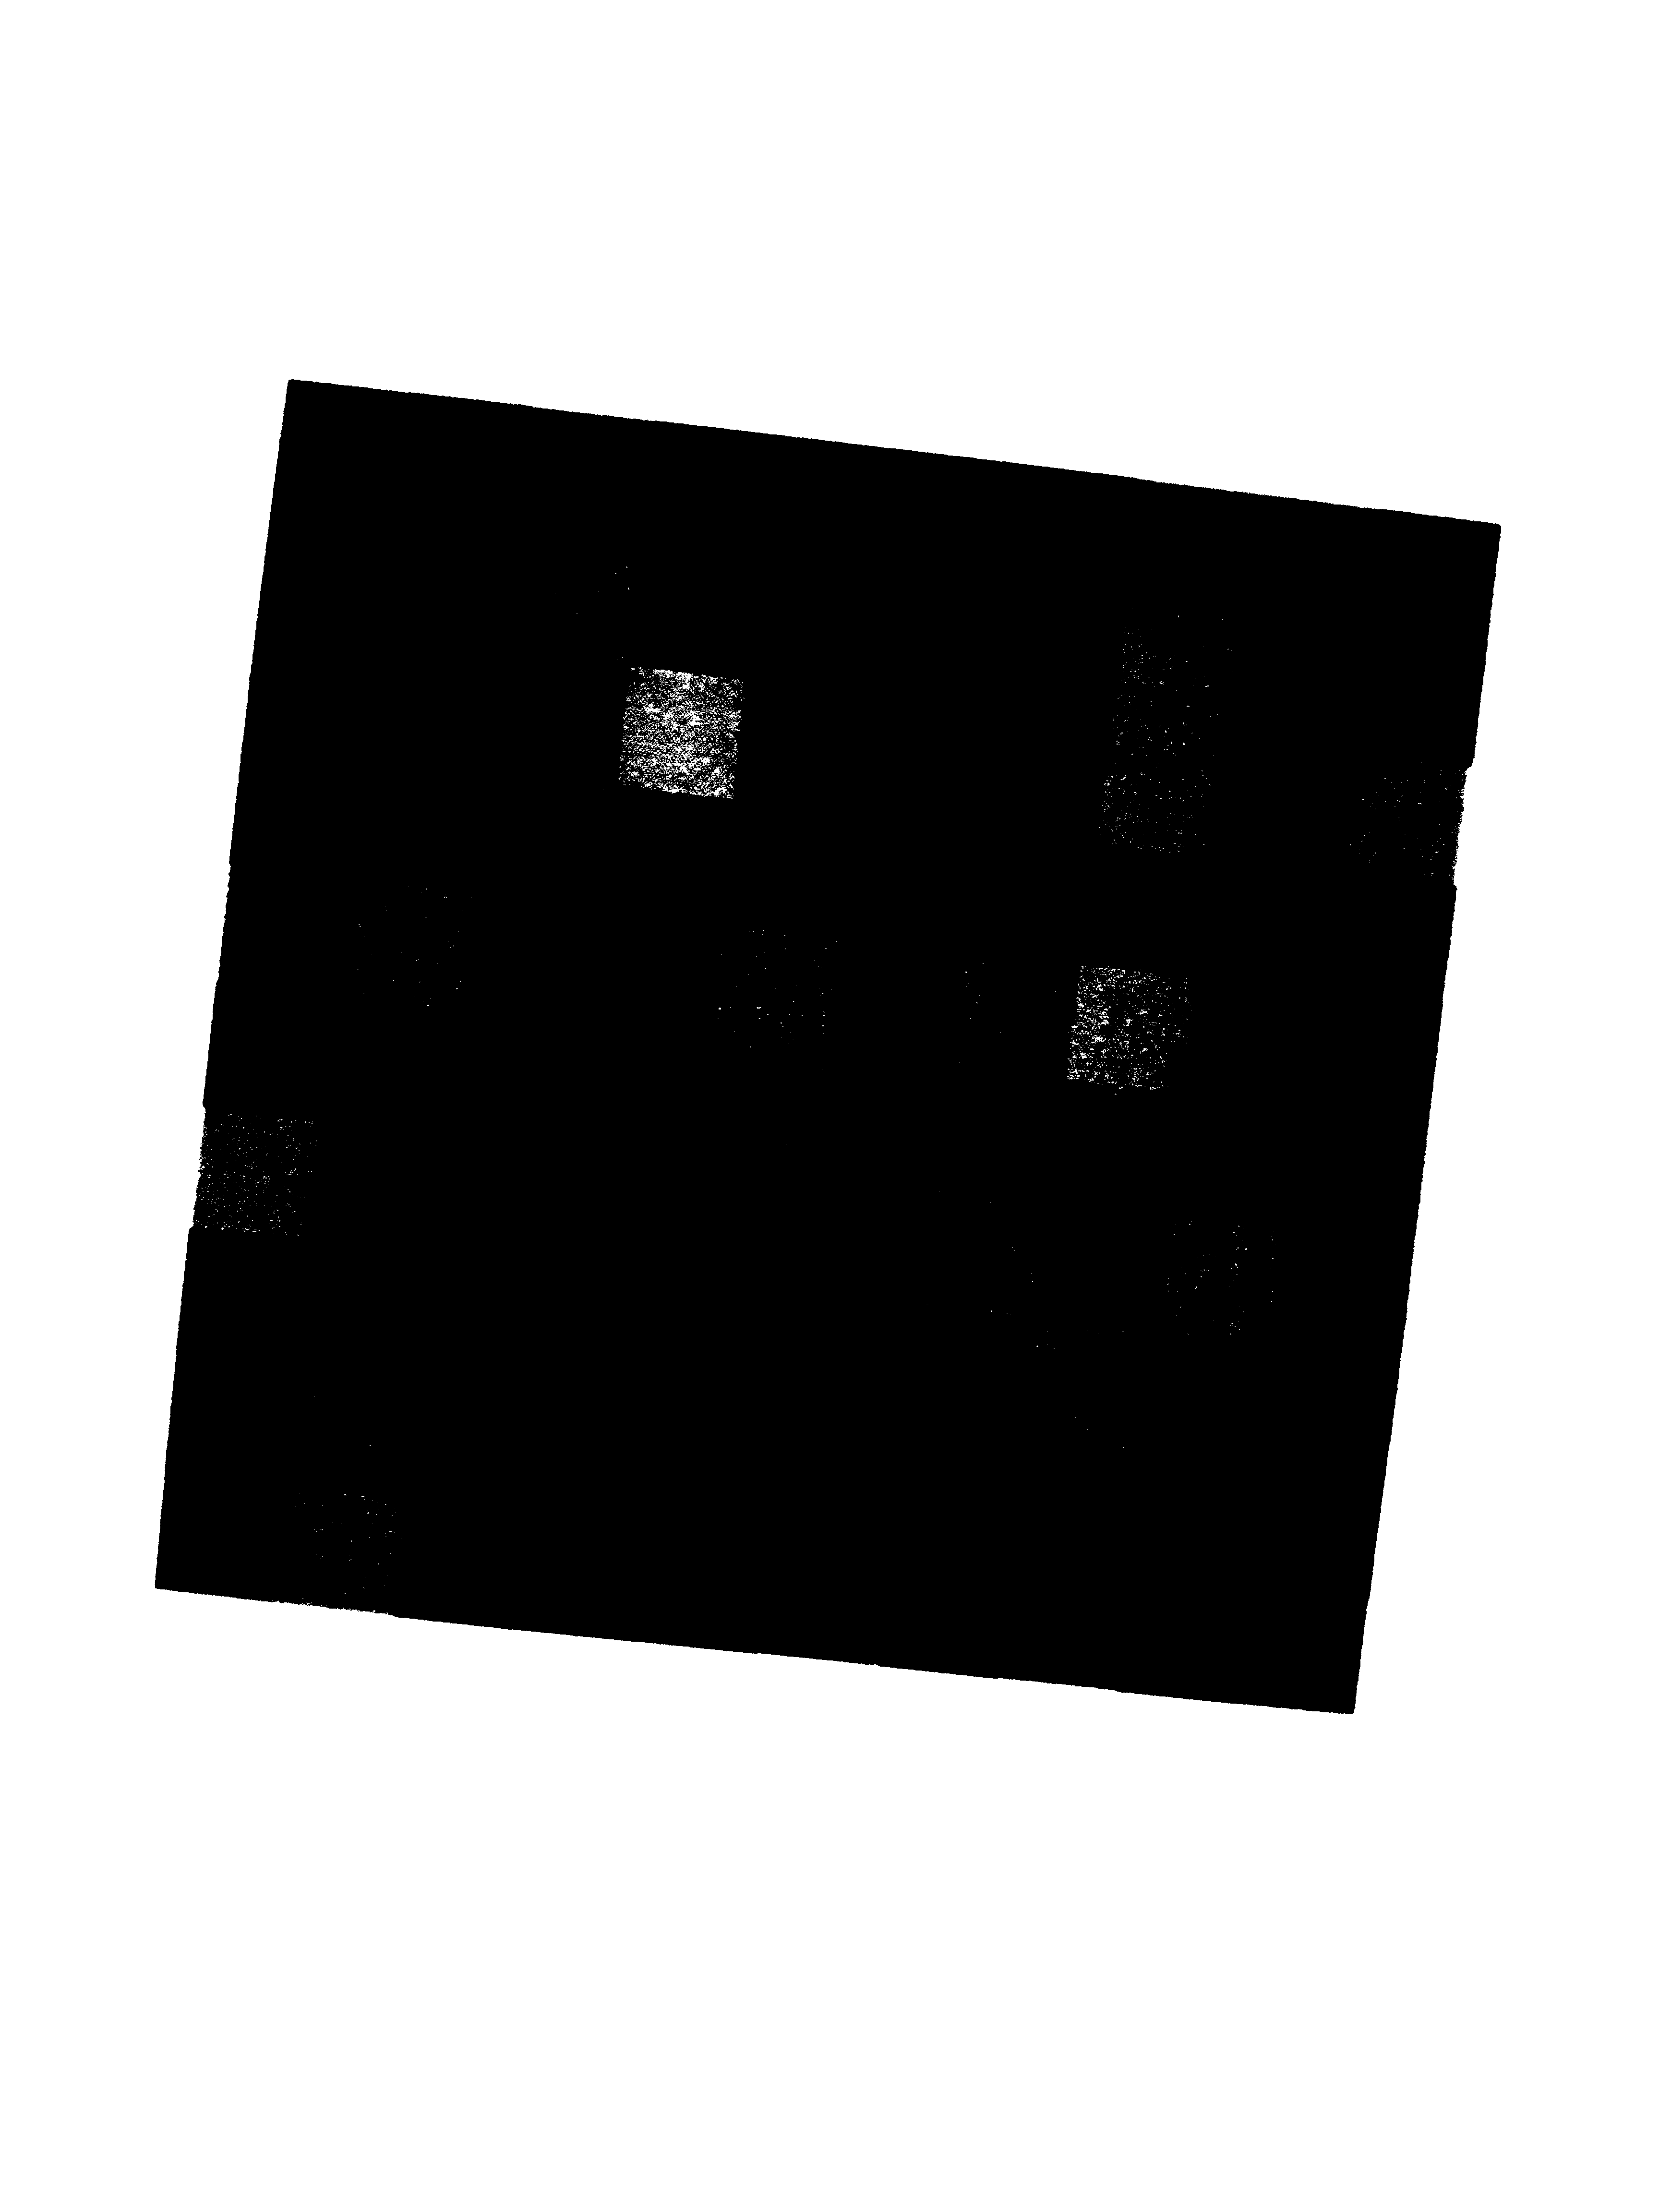
\includegraphics[width=0.3\textwidth]{rsc/binary.png}
                    \label{subfig:angle_binary}}
                \subfloat[Photo binaire avec angles retournés par l'algorithme]{
                    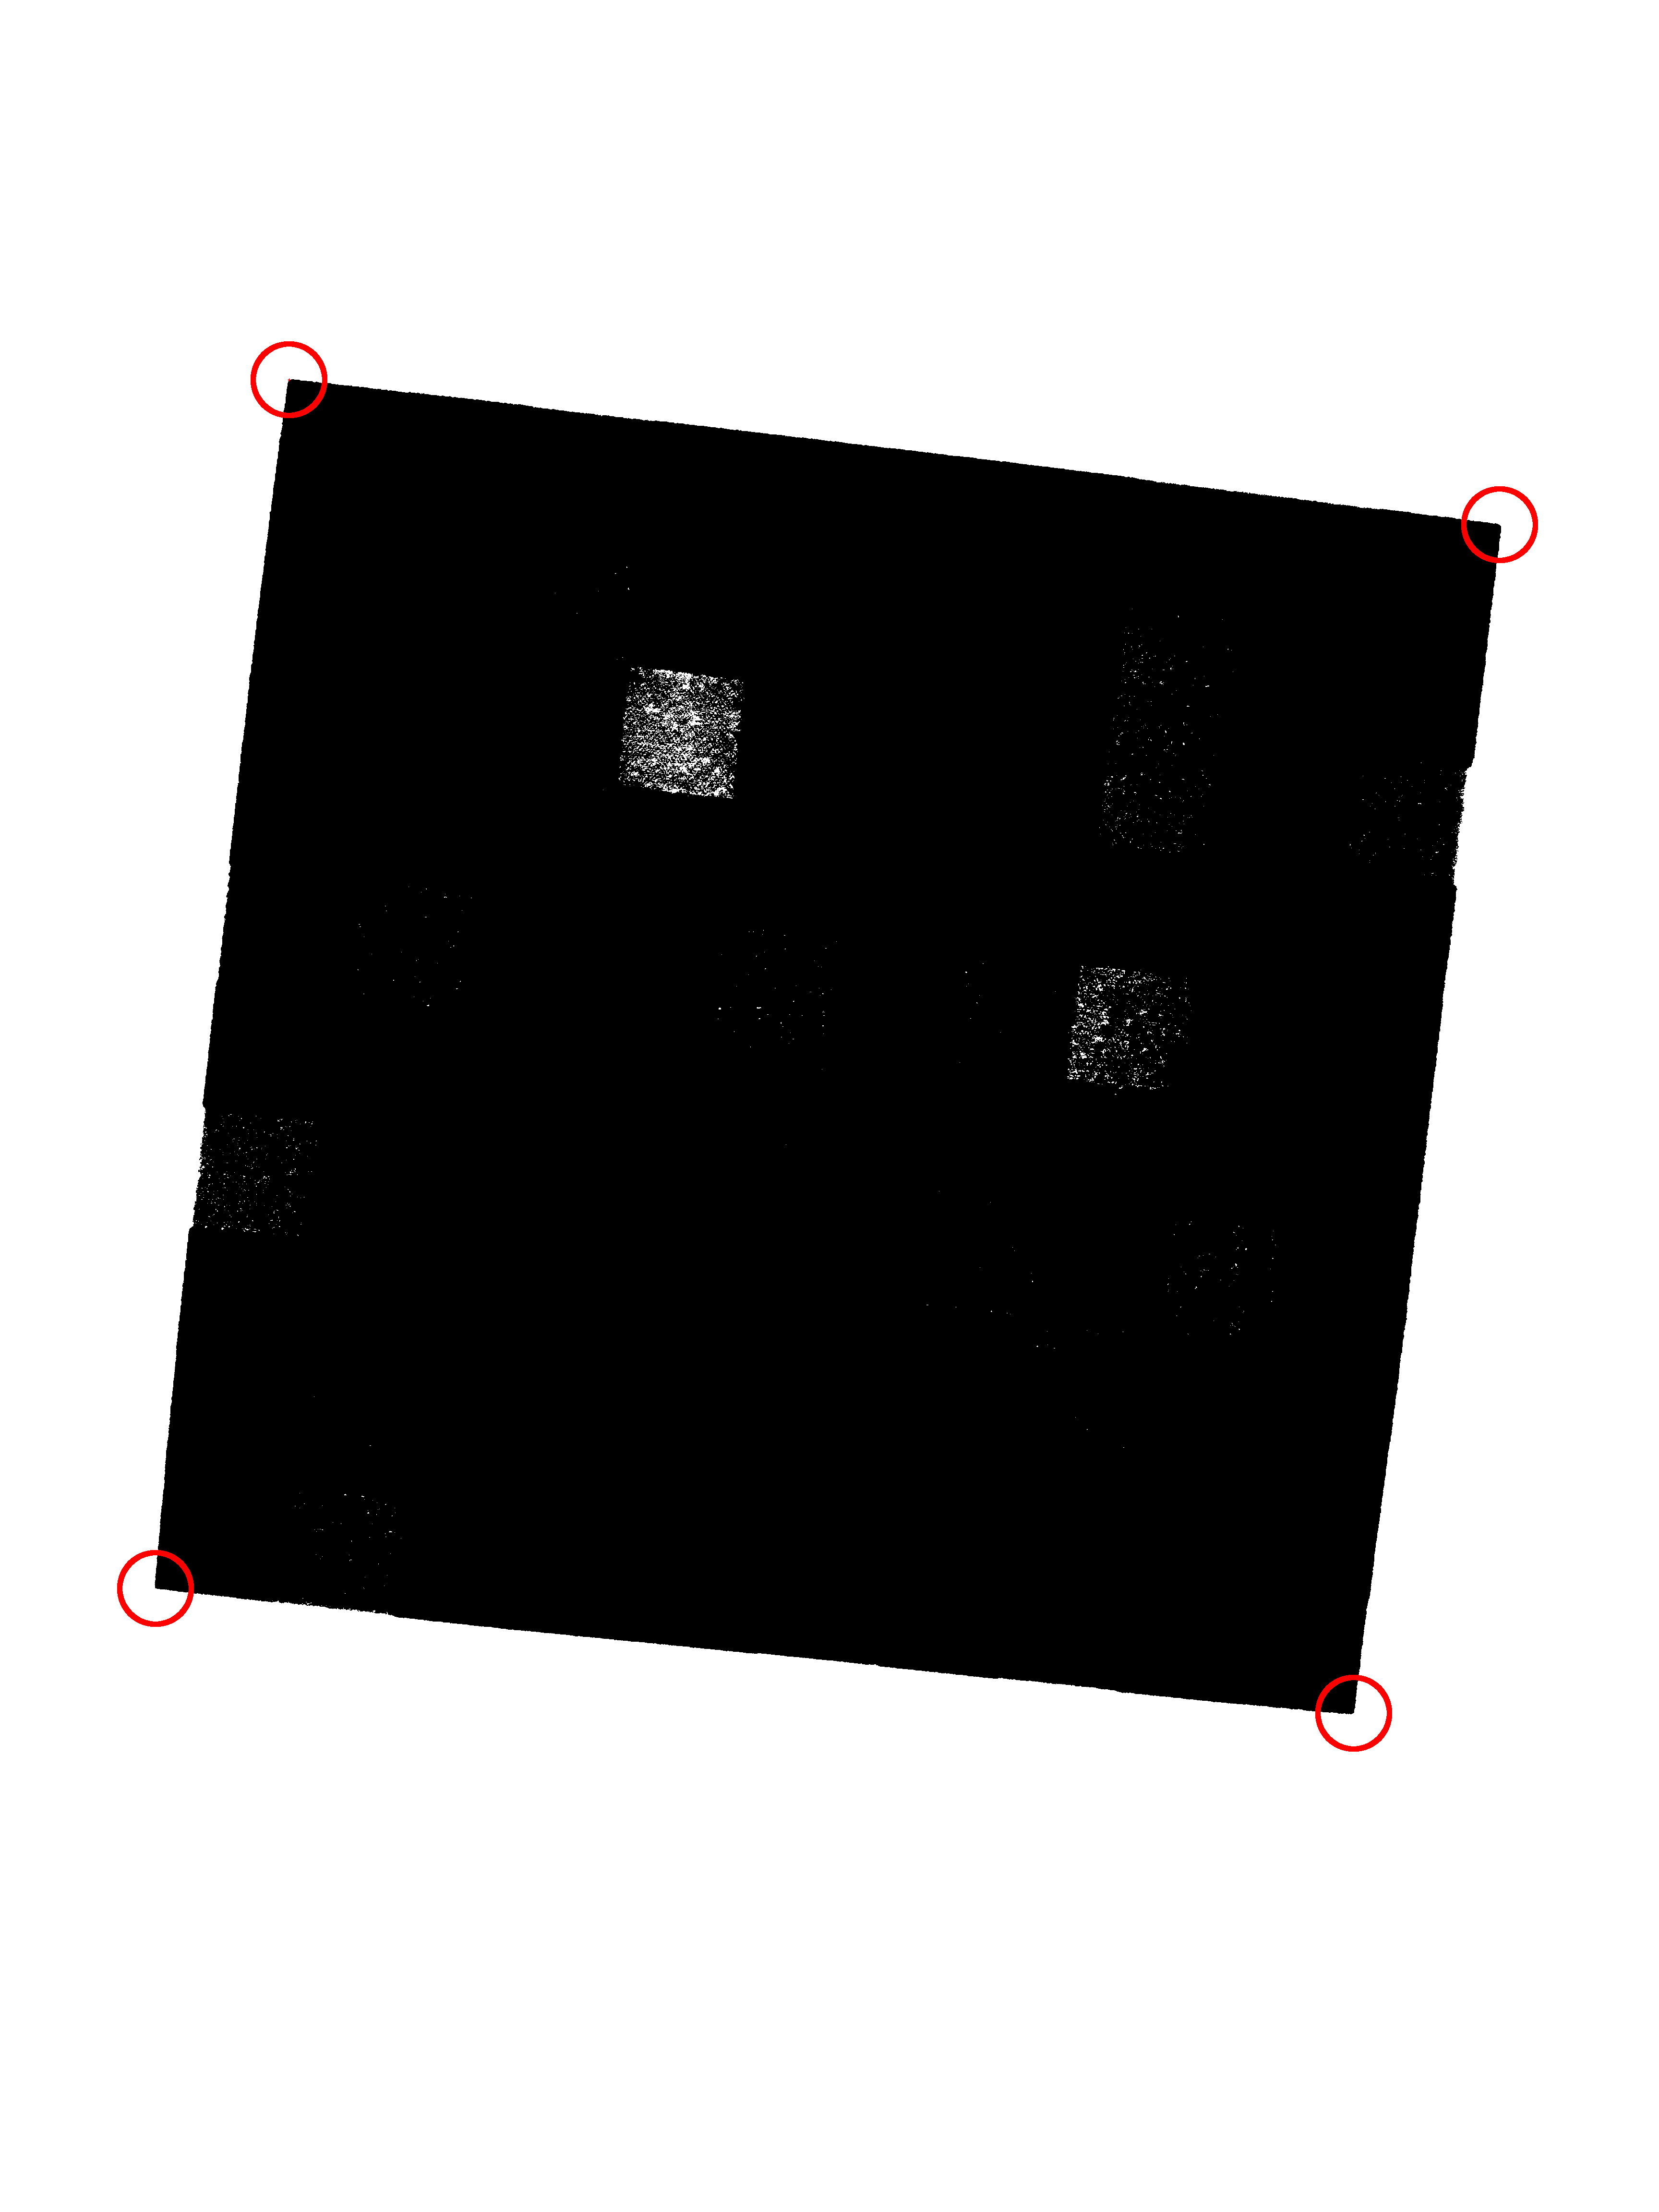
\includegraphics[width=0.3\textwidth]{rsc/findAngle.png}
                    \label{subfig:angle_res}}
                \caption{Détection des angles de la peinture sur l'image binaire}
                \label{fig:angle}
            \end{center}
        \end{figure}

        Pour que cet algorithme retourne les bonnes coordonnées pour chaque angle, il faut que l'image binaire ne présente aucun point noir en dehors de la zone centrale (la peinture). Pour empêcher cela, il faut soit choisir une valeur plus petite pour le seuillage de l'image (au risque de perdre des morceaux à l'intérieur ou sur les bords de la zone centrale), soit effectuer une ou plusieurs ouvertures (une érosion suivie d'une dilatation) pour supprimer les points isolés dans le fond de l'image sans toucher à la zone centrale.

    \section{Tranformation affine}

        Une fois que les angles de la peinture sont définis, il ne reste plus qu'une étape pour que l'image soit prête à être déchiffré. Il faut effectuer une transformation affine afin d'obtenir une image contenant uniquement la peinture positionnée correctement (les bords droits sans pente).

        Pour effectuer cette transformation, cinq points sont définis.
        \begin{itemize}
            \item E : point coulissant le long du coté supérieur
            \item F : point coulissant le long du coté gauche
            \item G : point coulissant le long du coté inférieur
            \item H : point coulissant le long du coté droit
            \item K : point d'intersection des segments EG et FH
        \end{itemize}

        Chacun des points E, F, G et H évolue sur une découpe de $n$ points d'un des côtés ($n$ correspondant aux dimensions de la nouvelle image).

        \begin{figure}[htbp]
            \begin{center}
                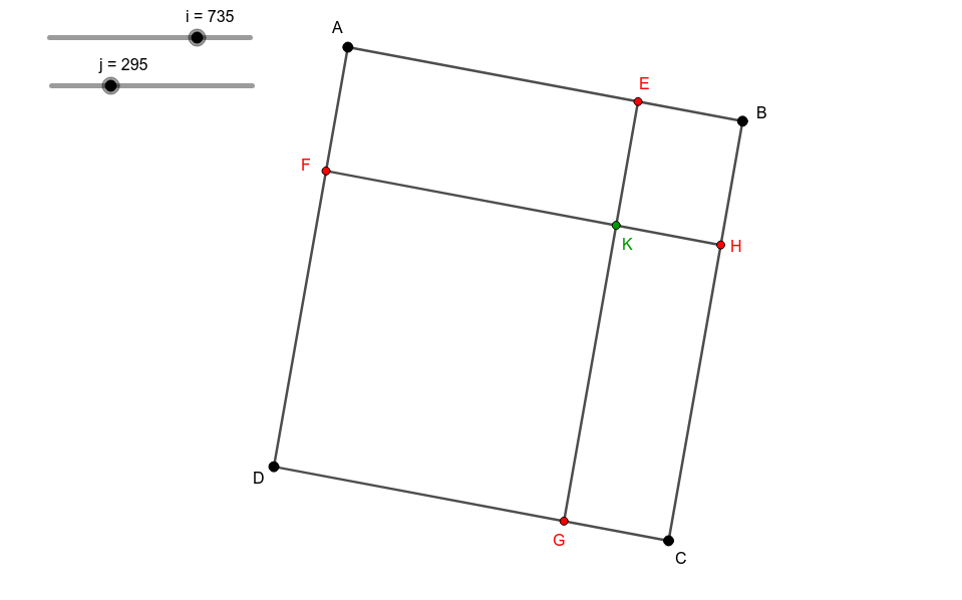
\includegraphics[width=0.5\textwidth]{rsc/formule.png}
                \caption{Calcul des coordonnées pour la transformation affine}
                \label{fig:transform}
            \end{center}
        \end{figure}

        Chaque pixel $[i,j]$ de la nouvelle image (transformée) est défini par une copie de la valeur aux coordonnées du point K pour les $i^{eme}$ points E/F et les $j^{eme}$ points F/H (cf. figure \ref{fig:transform}).

    \section{Résultats finaux}

        La figure \ref{fig:result} montre la totalité du processus de lecture et de déchiffrement d'une peinture à partir d'une photo.

        \begin{figure}[htbp]
            \begin{center}
                \subfloat[Photo de la peinture]{
                    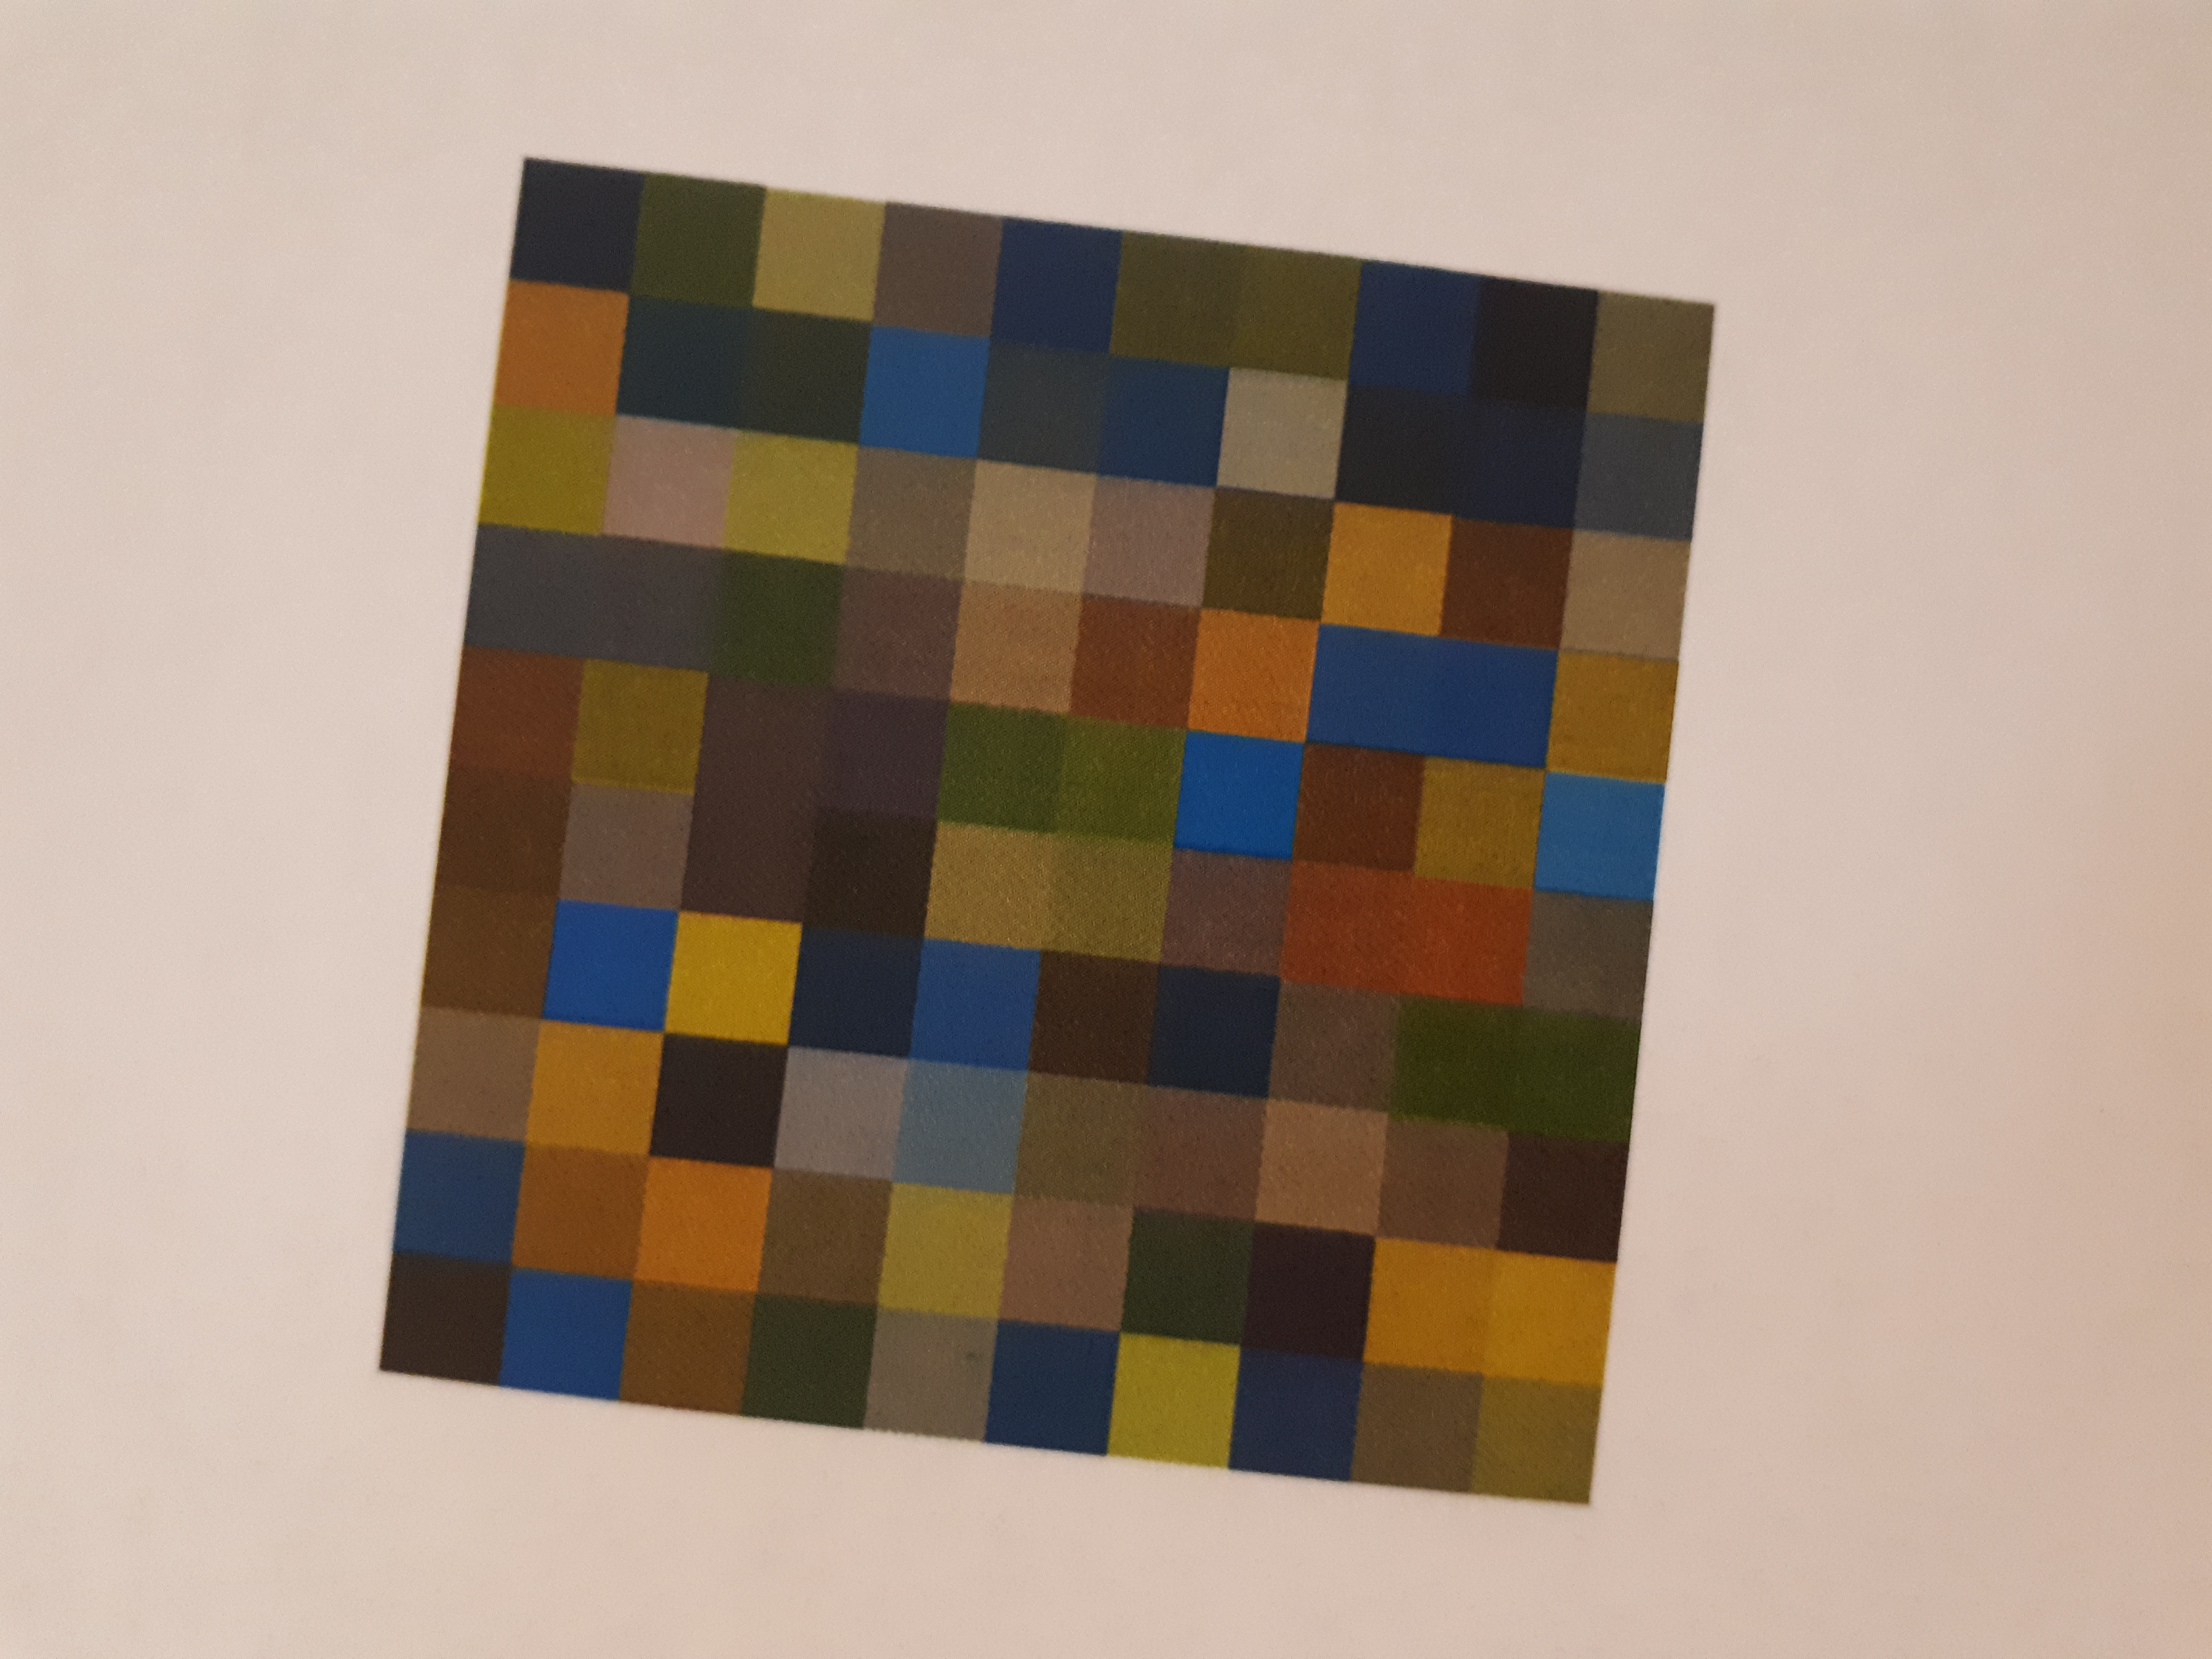
\includegraphics[width=0.3\textwidth]{rsc/vangogh.png}
                    \label{subfig:res_original}}
                \subfloat[Photo niveaux de gris]{
                    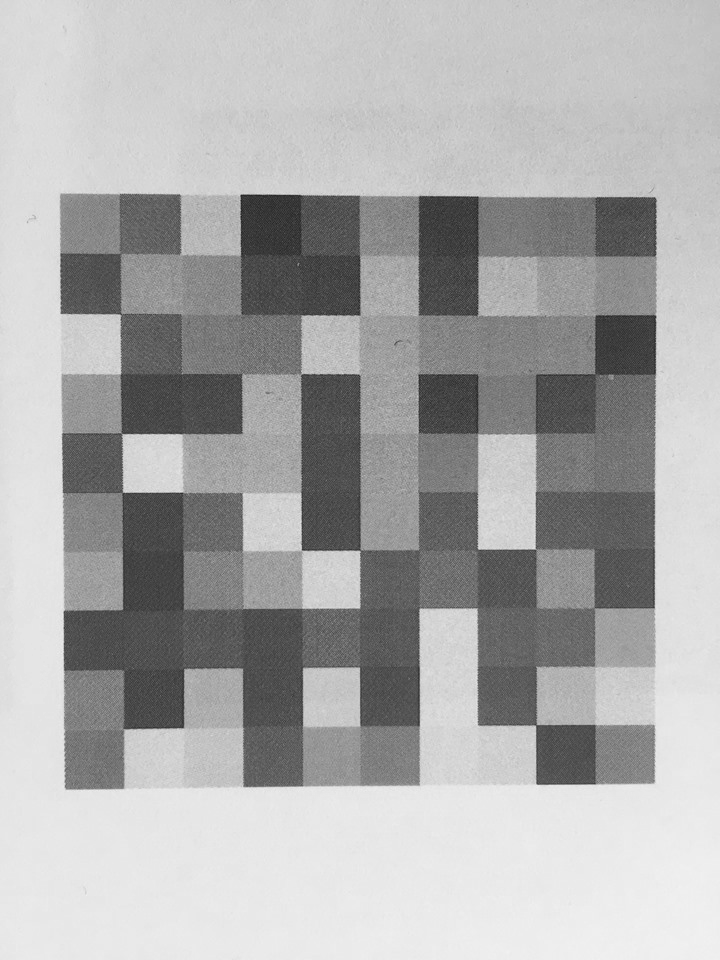
\includegraphics[width=0.3\textwidth]{rsc/grayScale.png}
                    \label{subfig:res_gray_scale}}
                \subfloat[Photo binaire binaire]{
                    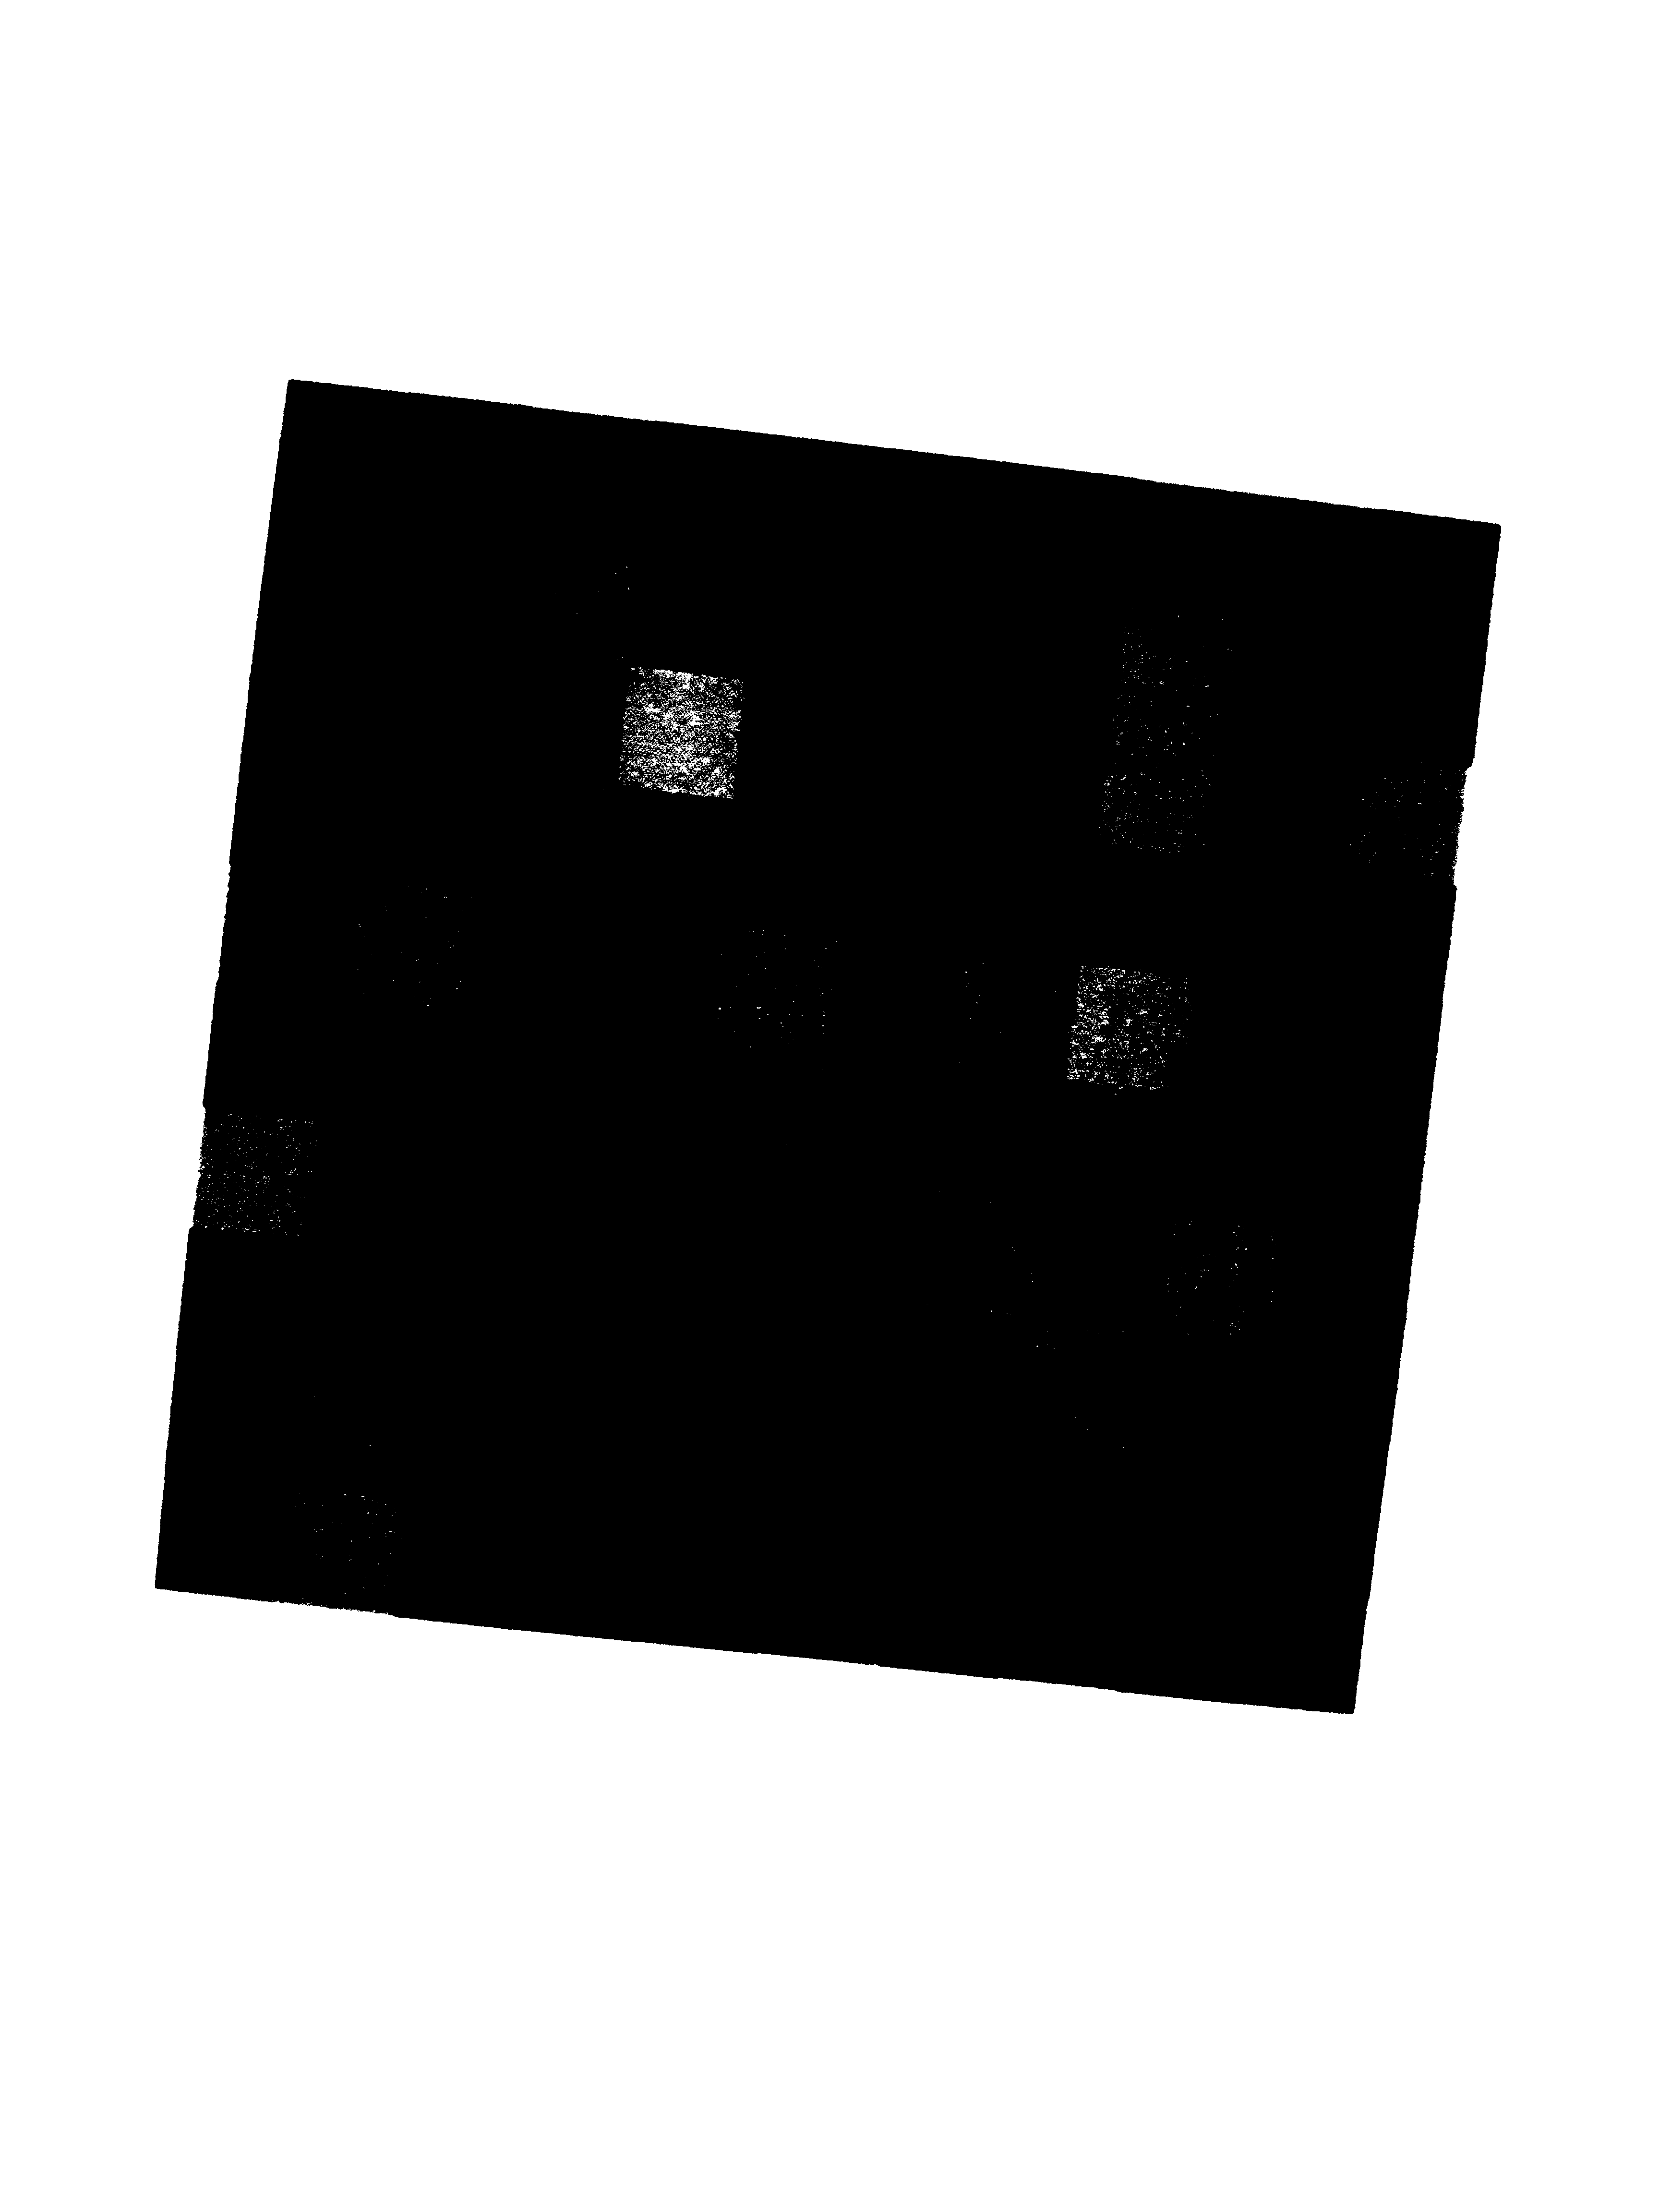
\includegraphics[width=0.3\textwidth]{rsc/binary.png}
                    \label{subfig:res_binary}}\\
                \subfloat[Détection des angles]{
                    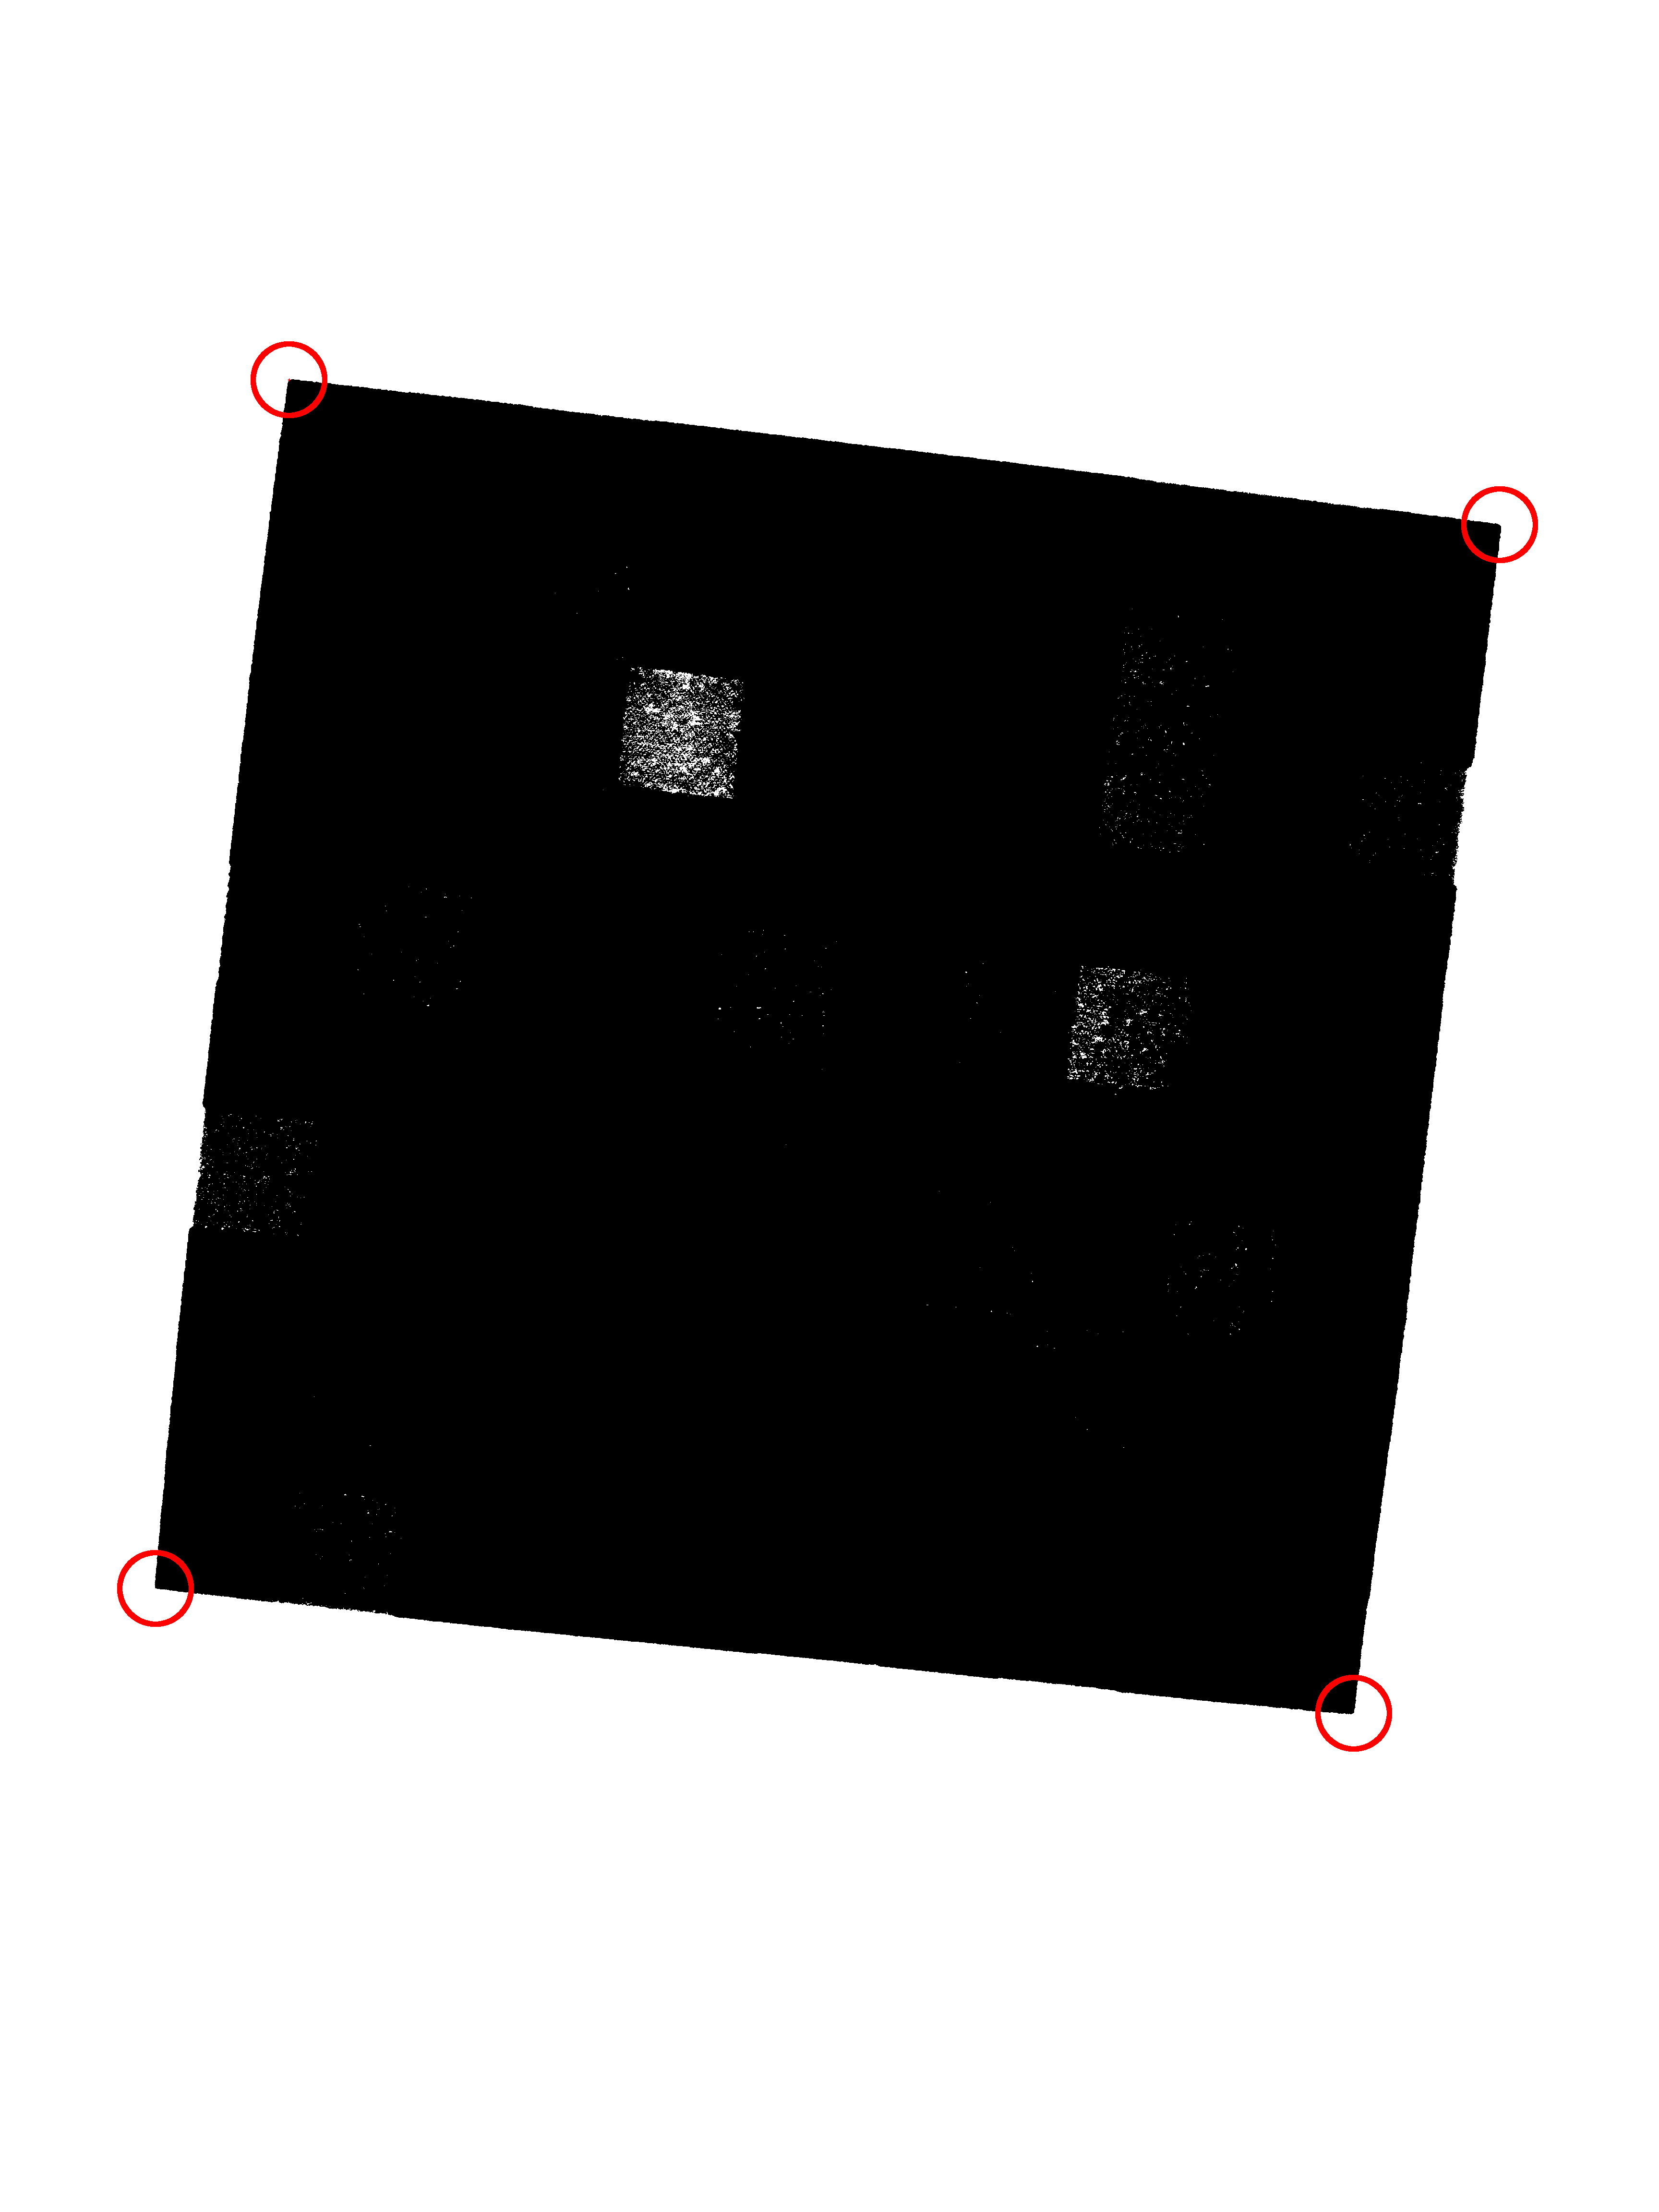
\includegraphics[width=0.3\textwidth]{rsc/findAngle.png}
                    \label{subfig:res_find_angle}}
                \subfloat[Transformation de l'image]{
                    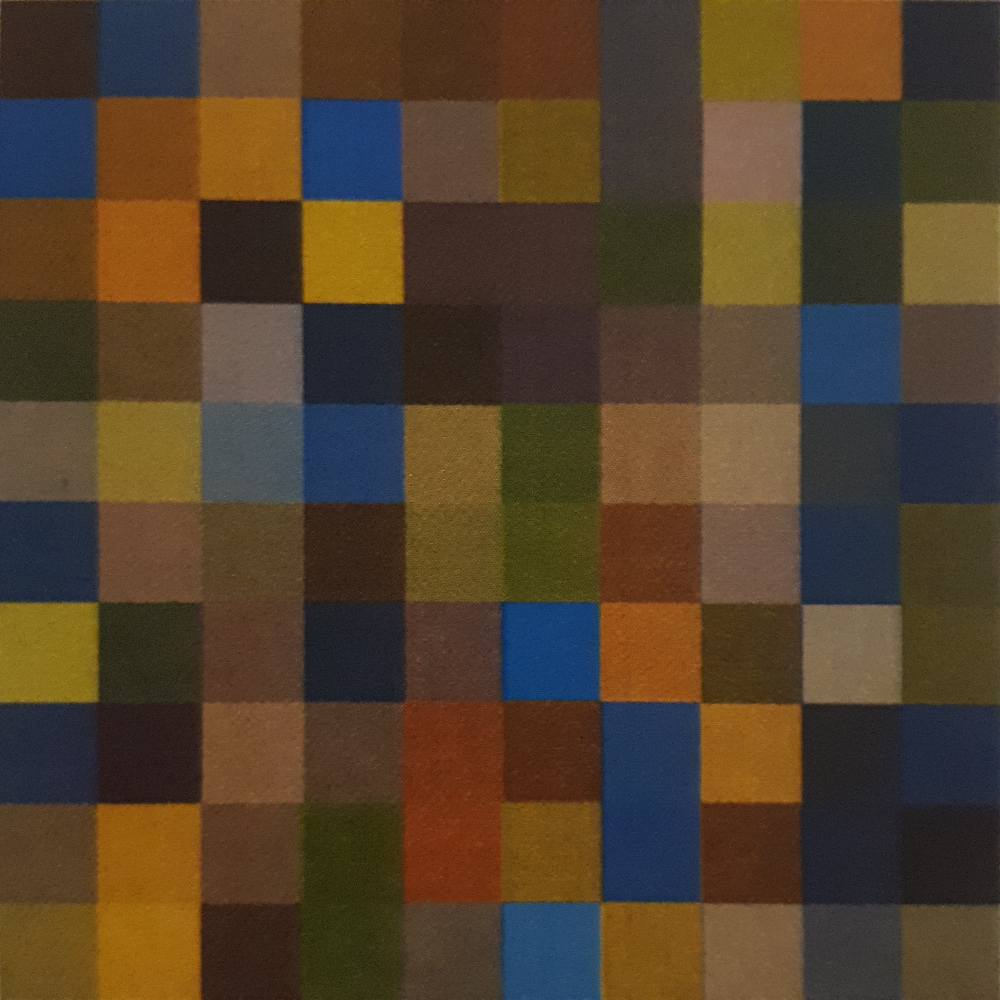
\includegraphics[width=0.3\textwidth]{rsc/transform.png}
                    \label{subfig:res_transform}}\\
                \subfloat[Déchiffrement de la photo]{
                    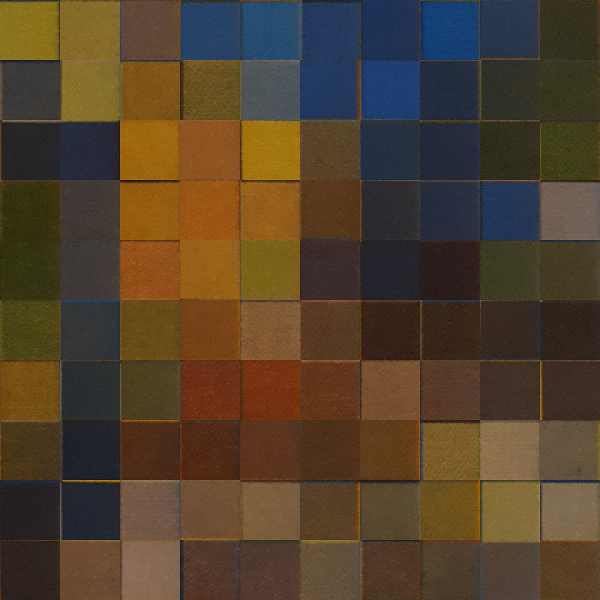
\includegraphics[width=0.3\textwidth]{rsc/decrypt.png}
                    \label{subfig:res_decrypt}}
                \subfloat[Déchiffrement attendu]{
                    
\includegraphics[width=0.3\textwidth]{rsc/decrypt_expected.png}
                    \label{subfig:res_decrypt_expected}}
                \caption{Résultat du processus total de déchiffrement de la peinture à partir d'une photo}
                \label{fig:result}
            \end{center}
        \end{figure}

\end{document}
